% Comments --

\documentclass{book}

\newcommand{\vect}[1]{{\bf{ #1}}}

\usepackage{epsfig}
\usepackage{graphicx}
%\usepackage[all]{xy}
%\usepackage{pb-diagram}

\title{An Introduction to Ray Tracing with JavaScript}


\author{Timothy J.~Hickey }
%\authorrunning{Hickey }
%\tocauthor{Timothy J.~Hickey (Brandeis University)}
%\institute{Computer Science Department, Brandeis University \\
%\email{\{tim}\@cs.brandeis.edu} }

\bibliographystyle{abbrv}

\begin{document}

%    \frontmatter

\maketitle
%    \include{titlepg}       % include title page
%    \include{preface}       % include preface
%    \include{other}         % include other frontmatter

%\begin{figure}[h]
%\centering
%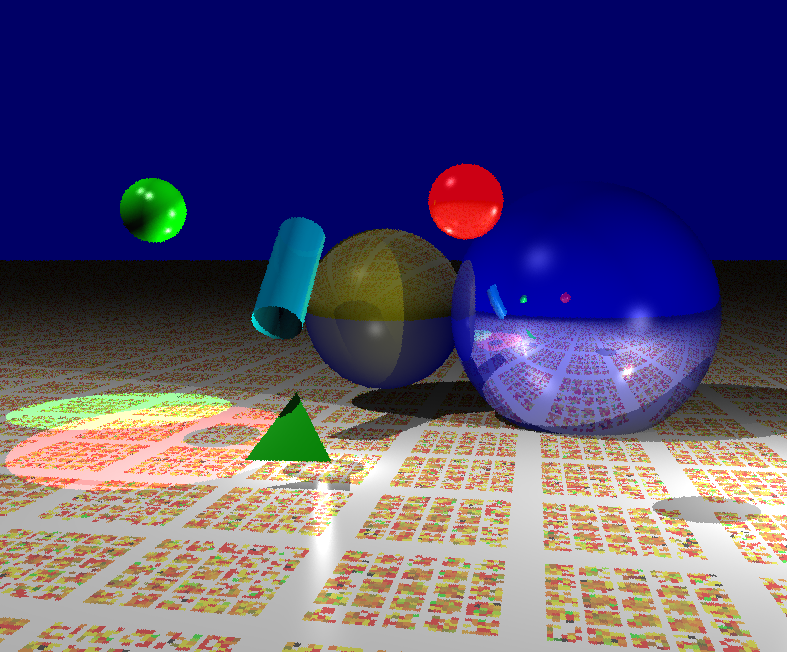
\includegraphics[width=5.5in]{images/cover.png}
%\end{figure}


 %   \mainmatter



\tableofcontents
%\newpage

\chapter*{Acknowledgements}
Many thanks to the students in my CS155b Computer Graphics classes for finding typos and suggesting improvements to these notes!

\chapter{Introduction}
These notes provide an introduction to RayTracing.  There are no prerequisites beyond high school mathematics (geometry, algebra, trigonometry, analytic geometry) assumed for reading these notes, except for an occasional bit of linear algebra, most of which we explain from basic principles.  On the other hand, the programming exercises assume you know how to program in some object-oriented language and that you can find and read APIs for that language. For example, Java, C\#, C++, Ruby, Python, Javascript, etc. are all reasonable languages to use when implementing your ray tracer.



\section{Ray Tracing}
Ray Tracing is a method of generating realistic 3D images from a mathematical description of a scene. The basic idea
is that one creates a 3D scene consisting of a camera, lights, and various 3D objects, such as sphere, planes, cylinders,
or polyhedra. Next one generates a 2d image on the screen that represents the view of that 3D scene from the camera. The view is generated by associating to each pixel in the screen window a ray that starts at the camera and moves out in a straight line into the
scene. Using simple (and fast) mathematical tests, one determines the first object that the ray intersects and then
determines the color of that pixel by using the properties of the lights and materials. One can obtain more realistic
images by letting the ray reflect off of the partly mirrored object and refract through the partly transparent objects.
The reflected and refracted light must then be combined in a weighted average with the already computed material color.

In these notes we will describe the mathematics and algorithms behind ray tracing and in the process guide you in the development of a simple
ray tracer in the language of your choice. The image below is an example of your ray tracer will be able to produce:
\begin{figure}[h]
\centering
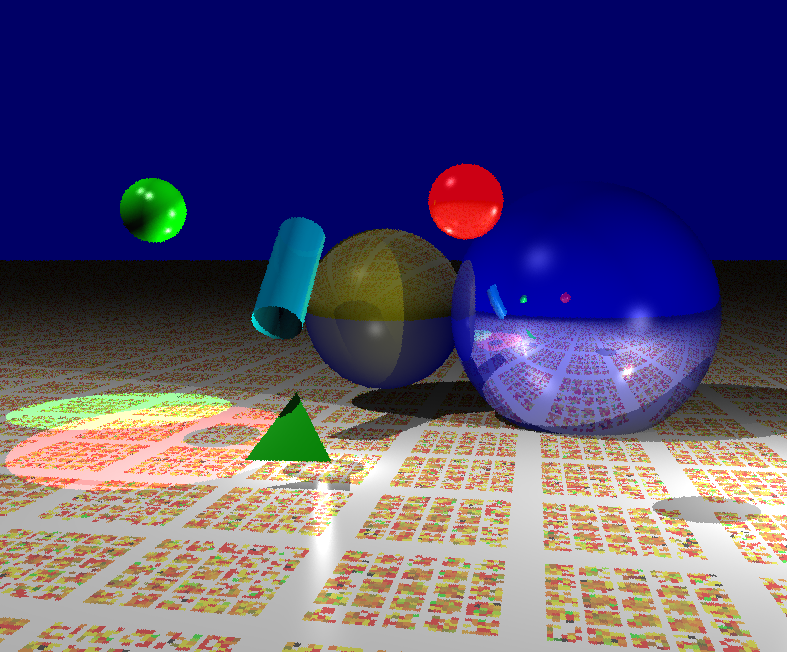
\includegraphics[width=4in]{images/cover.png}
\end{figure}

We begin the notes with some preliminaries about points, vectors and rays in 3D space.

\chapter{Points and Rays \label{chap:prelim}}

\section{3D coordinates}
Any point $\vect{a}$ in 3D space can be uniquely described by giving its 3D coordinates $\vect{a}=(a_x, a_y, a_z)$
which describe the distance to $a$ in each of the three directions corresponding to the $x$, $y$, and $z$ axes.

\begin{figure}[h]
\centering
\includegraphics[width=2.5in]{images/point3D.jpg}
\caption{3D coordinates}
\end{figure}



Each point $\vect{a}$ uniquely defines a directed line segment from the origin $(0,0,0)$ to $\vect{a}$.
We call such directed line segments vectors and we will often switch back and forth between these two
interpretations of $\vect{a}$.


For example,
the distance $\vert\vect{a}\vert$ of a point $\vect{a}$ from the origin $(0,0,0)$ is also the
length of the vector $\vect{a}$
and which is computed using a generalized pythagorean theorem:
\begin{eqnarray}
\vert\vect{a}\vert &=& \sqrt{a_x^2 + a_y^2 + a_z^2}
\label{eqn:genpyth}
\end{eqnarray}

\subsection{Proof of the Pythagorean Theorem}
Lets prove the generalized pythagorean theorem (Eq \ref{eqn:genpyth}) by starting with a simple
geometric proof of the 2 dimensional Pythagorean theorem. Remember, this states that if a right triangle
has sides of length $A$, $B$, and $C$ with $C$ being the hypotenuse, then $A^2 + B^2 = C^2$.

This can be easily demonstrated using the diagram in Figure \ref{fig:pyth2da}.

\begin{figure}[h]
\centering
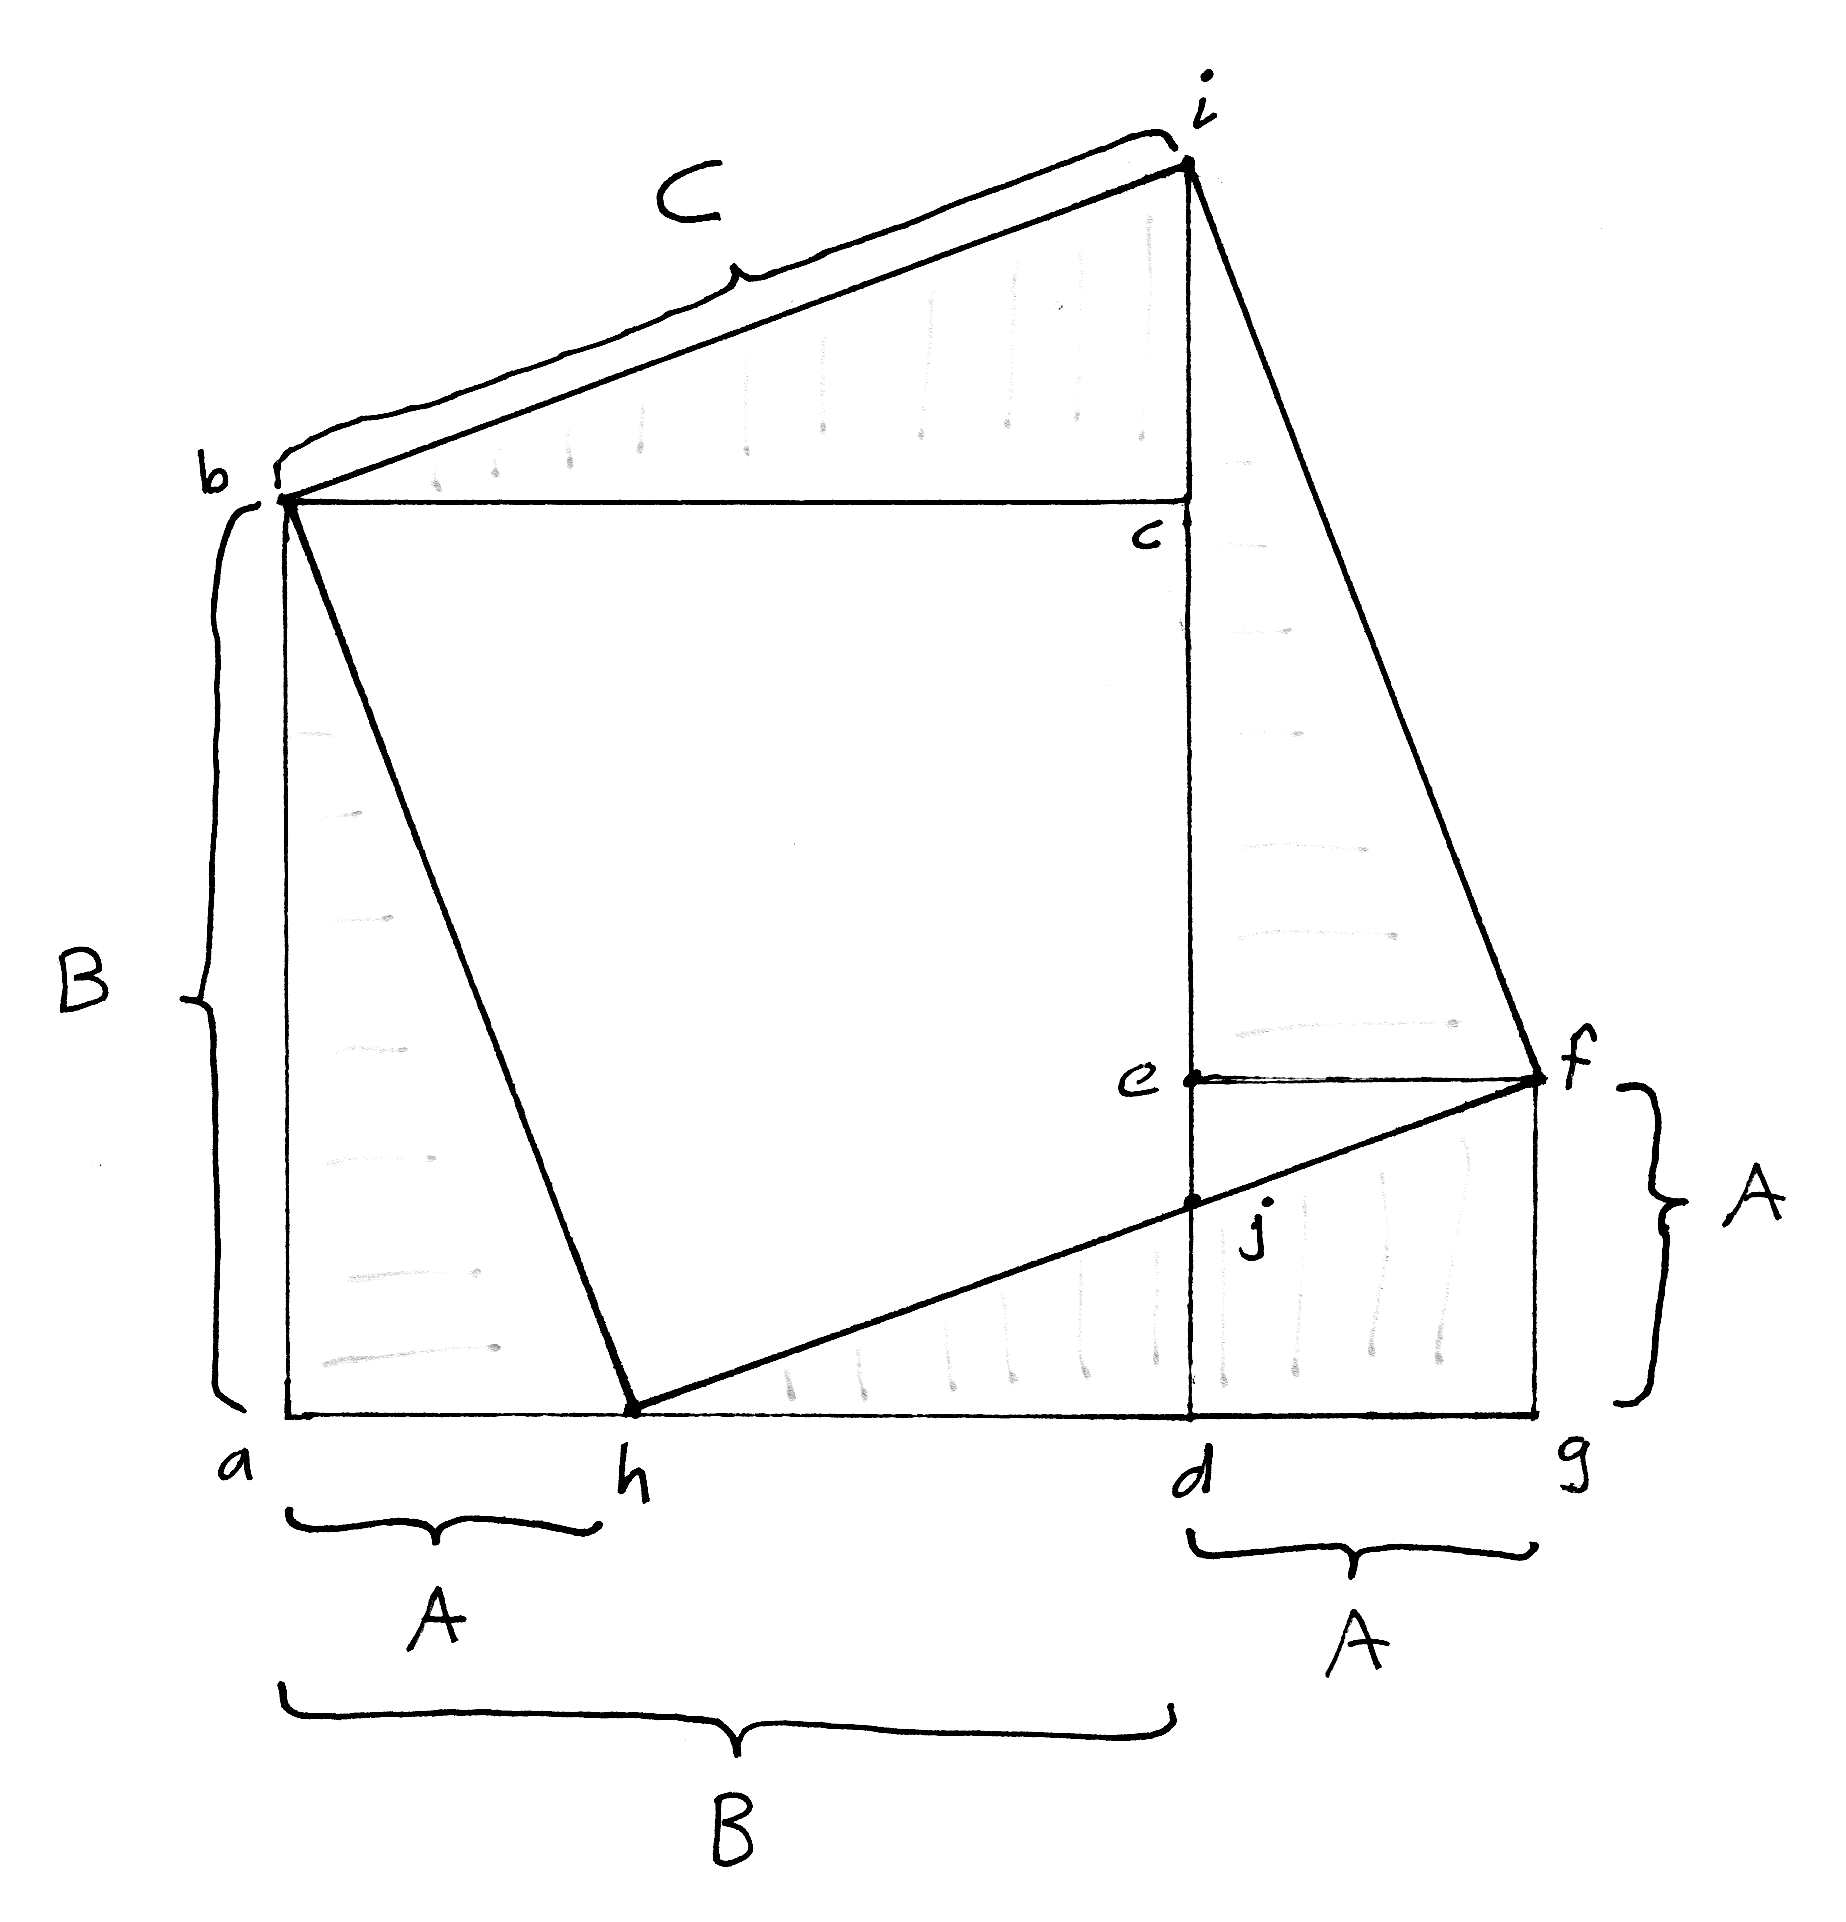
\includegraphics[width=2.5in]{images/pyth2da.jpg}
\caption{Pythagorean Theorem \label{fig:pyth2da}}
\end{figure}

Observe that $A^2+B^2$ is the area of the two squares $abcd$ and $defg$. The clever idea here is to
cut out two right triangles $\triangle ahb$ and $\triangle gfh$ with sides $A,B,C$ from these two squares and to move them to
$\triangle cib$ and $\triangle efi$ respectively.  Note that we can move them just by rotating them 90 degrees around the points $b$ and $f$ respectively.  Moving these two triangles changes the shape from the union of two squares
($abcd$ and $defg$) into the single quadrilateral $bhfi$ whose sides are all of length $C$. If we can prove
that this quadilateral is a square, then its area will be $C^2$ and we will have shown that $A^2+B^2=C^2$
for a right triangle of sides $A,B$ and hypotenuse $C$. So we need to prove that each of the four angles
of the quadrilateral are right angles, but this follows easily from the fact that the sum of the angles
of a triangle is 180 degrees and hence the sum of the two non-right angles is 90 degrees. For example,
\[
\angle fib = \angle fic + \angle cib = \angle ibc + \angle cib = 90^\circ
\]
and we leave the other three angles as geometry exercises.
Q.E.D.

\subsection{Proof of the Generalized Pythagorean Theorem}

We can prove the 3 dimensional pythagorean theorem by applying the 2d version twice. Indeed,
consider the figure below. We let $\vect {p} = (p_x, p_y, p_z)$ be an arbitrary 3D point and
let $\vect q = (p_x, 0, p_z)$ be its projection into the $xz$ plane. Observe that the line
segment from the origin to $\vect{q}$ is the hypotenuse of a right triangle in the $xz$-plane
whose sides have lengths $p_x$ and $p_z$. Thus we can apply the 2d pythagorean theorem
to determine the length $h_1$ of the vector $\vect{q}$:
\[
h_1 = \sqrt{p_x^2 + p_z^2}
\]
Now consider the three points $p$, $q$, and the origin $o$. These three points uniquely determine a
plane and it's clear that then angle $\angle oqp$ is a right angle (since the $y$-axis is perpendicular
to the $xz$ plane). Thus, we can again apply the 2d pythagorean theorem and we obtain the length
$h_2$ of the vector $\vect {p}$
\[
h_2^2 = h_1^2 + p_y^2 = p_x^2 + p_z^2 + p_y^2 = p_x^2 + p_y^2 + p_z^2
\]

\begin{figure}[h]
\centering
\includegraphics[width=2.5in]{images/pyth3D.jpg}
\caption{Length of a vector in 3D \label{fig:pyth3D}}
\end{figure}

A similar proof would work in dimensions 4 and more by inductively projecting down 1 dimension,
applying the $n-1$ dimensional pythagorean theorem and then completing the induction step using
the 2d pythagorean theorem in the 2d plane consisting of the origin, the point, and its projection
into an $n-1$ dimensional subspace.

\section{Dot products, norms, and vector lengths}
Given two vectors  ${\vect p} = (p_x, p_y, p_z)$
and ${\vect q} = (q_x, q_y, q_z)$.
Their dot-product is denoted ${\vect p} \cdot {\vect q}$ and is defined by
\[
{\vect p} \cdot {\vect q} = (p_x*q_x + p_y*q_y + p_z*q_z)
\]
The norm of a vector is defined to be the square root of its dot product with itself:
\[
\vert {\vect p} \vert = \sqrt{{\vect p} \cdot {\vect p}} = \sqrt{(p_x^2 + p_y^2 + p_z^2)}
\]
which, as we have seen, is the length of the vector:
\[
\vert {\vect p} \vert = \sqrt{(p_x^2 + p_y^2 + p_z^2)}
\]
A vector whose length is 1 is called ``normalized''
Any vector ${\vect v}$ can be normalized by dividing by its length:
\[
\frac {{\vect v} } {\vert {\vect v} \vert}
\]

\subsection{Geometric Interpretation of the Dot Product}
In this section, we show that if ${\vect u}$ and ${\vect v}$ are two vectors, then
\begin{eqnarray}
{\vect u} \cdot {\vect v} = \cos(\theta) \vert \vect{u} \vert  \vert \vect{v} \vert
\label{eqn:dotprod}
\end{eqnarray}
where $\theta$ is the angle between $\vect{u}$ and $\vect{v}$.

We can get a geometric interpretation of this property by considering the figure below.
Let $u$ and $v$ be two vectors and assume that $u$ is normalized (i.e. $\vert \vect{u}\vert = 1$).
Then as the figure shows the projection of $v$ onto $u$ is a vector of length $\cos(\theta) \vert\vect{v}\vert$.

\begin{figure}[h]
\centering
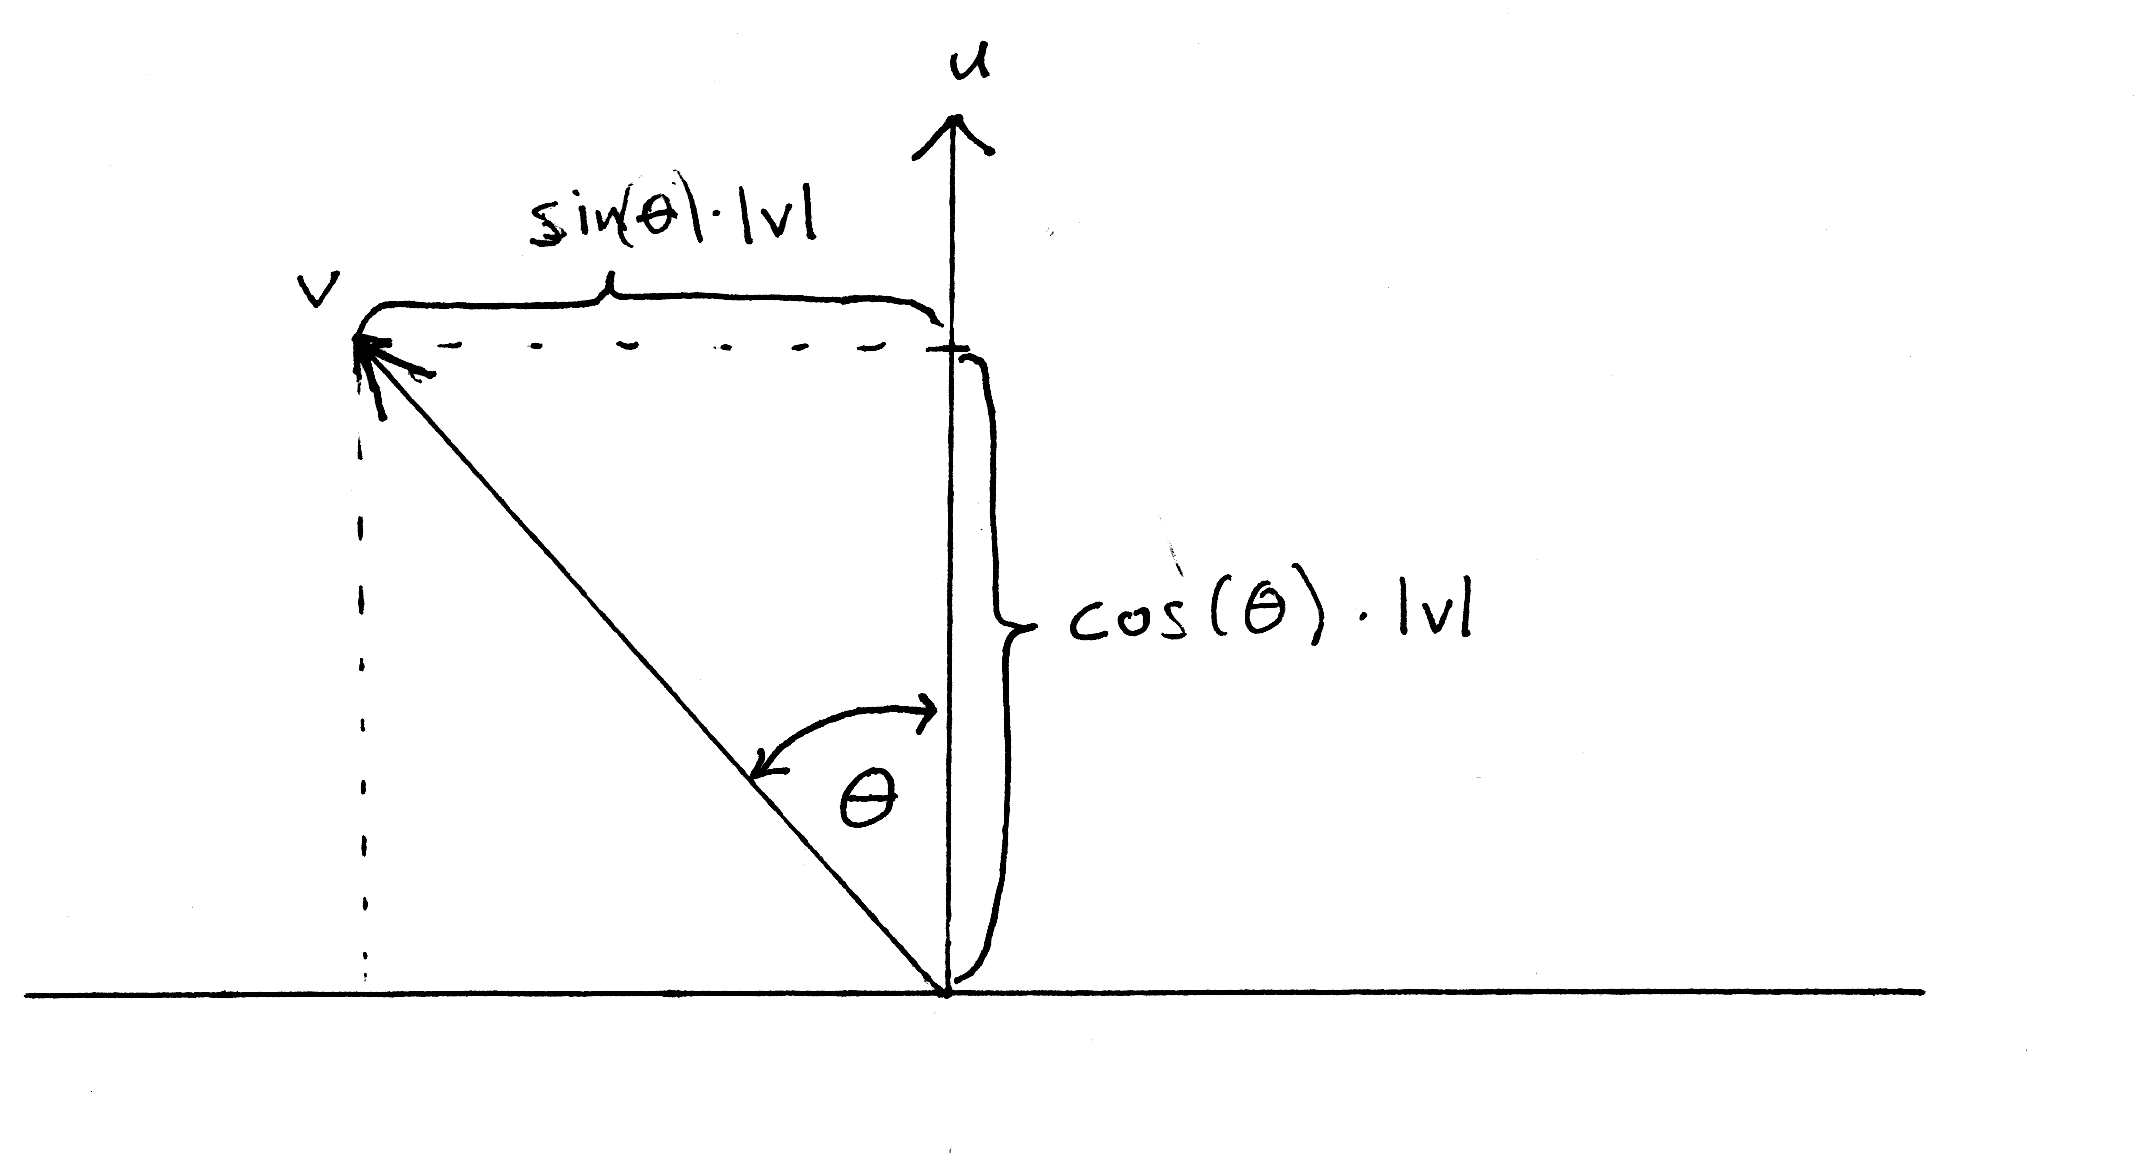
\includegraphics[width=2.5in]{images/projection.jpg}
\caption{$\vert v \vert \; \cos (\theta)$ is the projection of $\vect{v}$ on $\vect{u}$}
\end{figure}

To prove the property of the dot product in Eqn \ref{eqn:dotprod},
 we need to first recall and prove the Law of Cosines
which is a generalization of the pythagorean theorem for general triangles.

\begin{figure}[h]
\centering
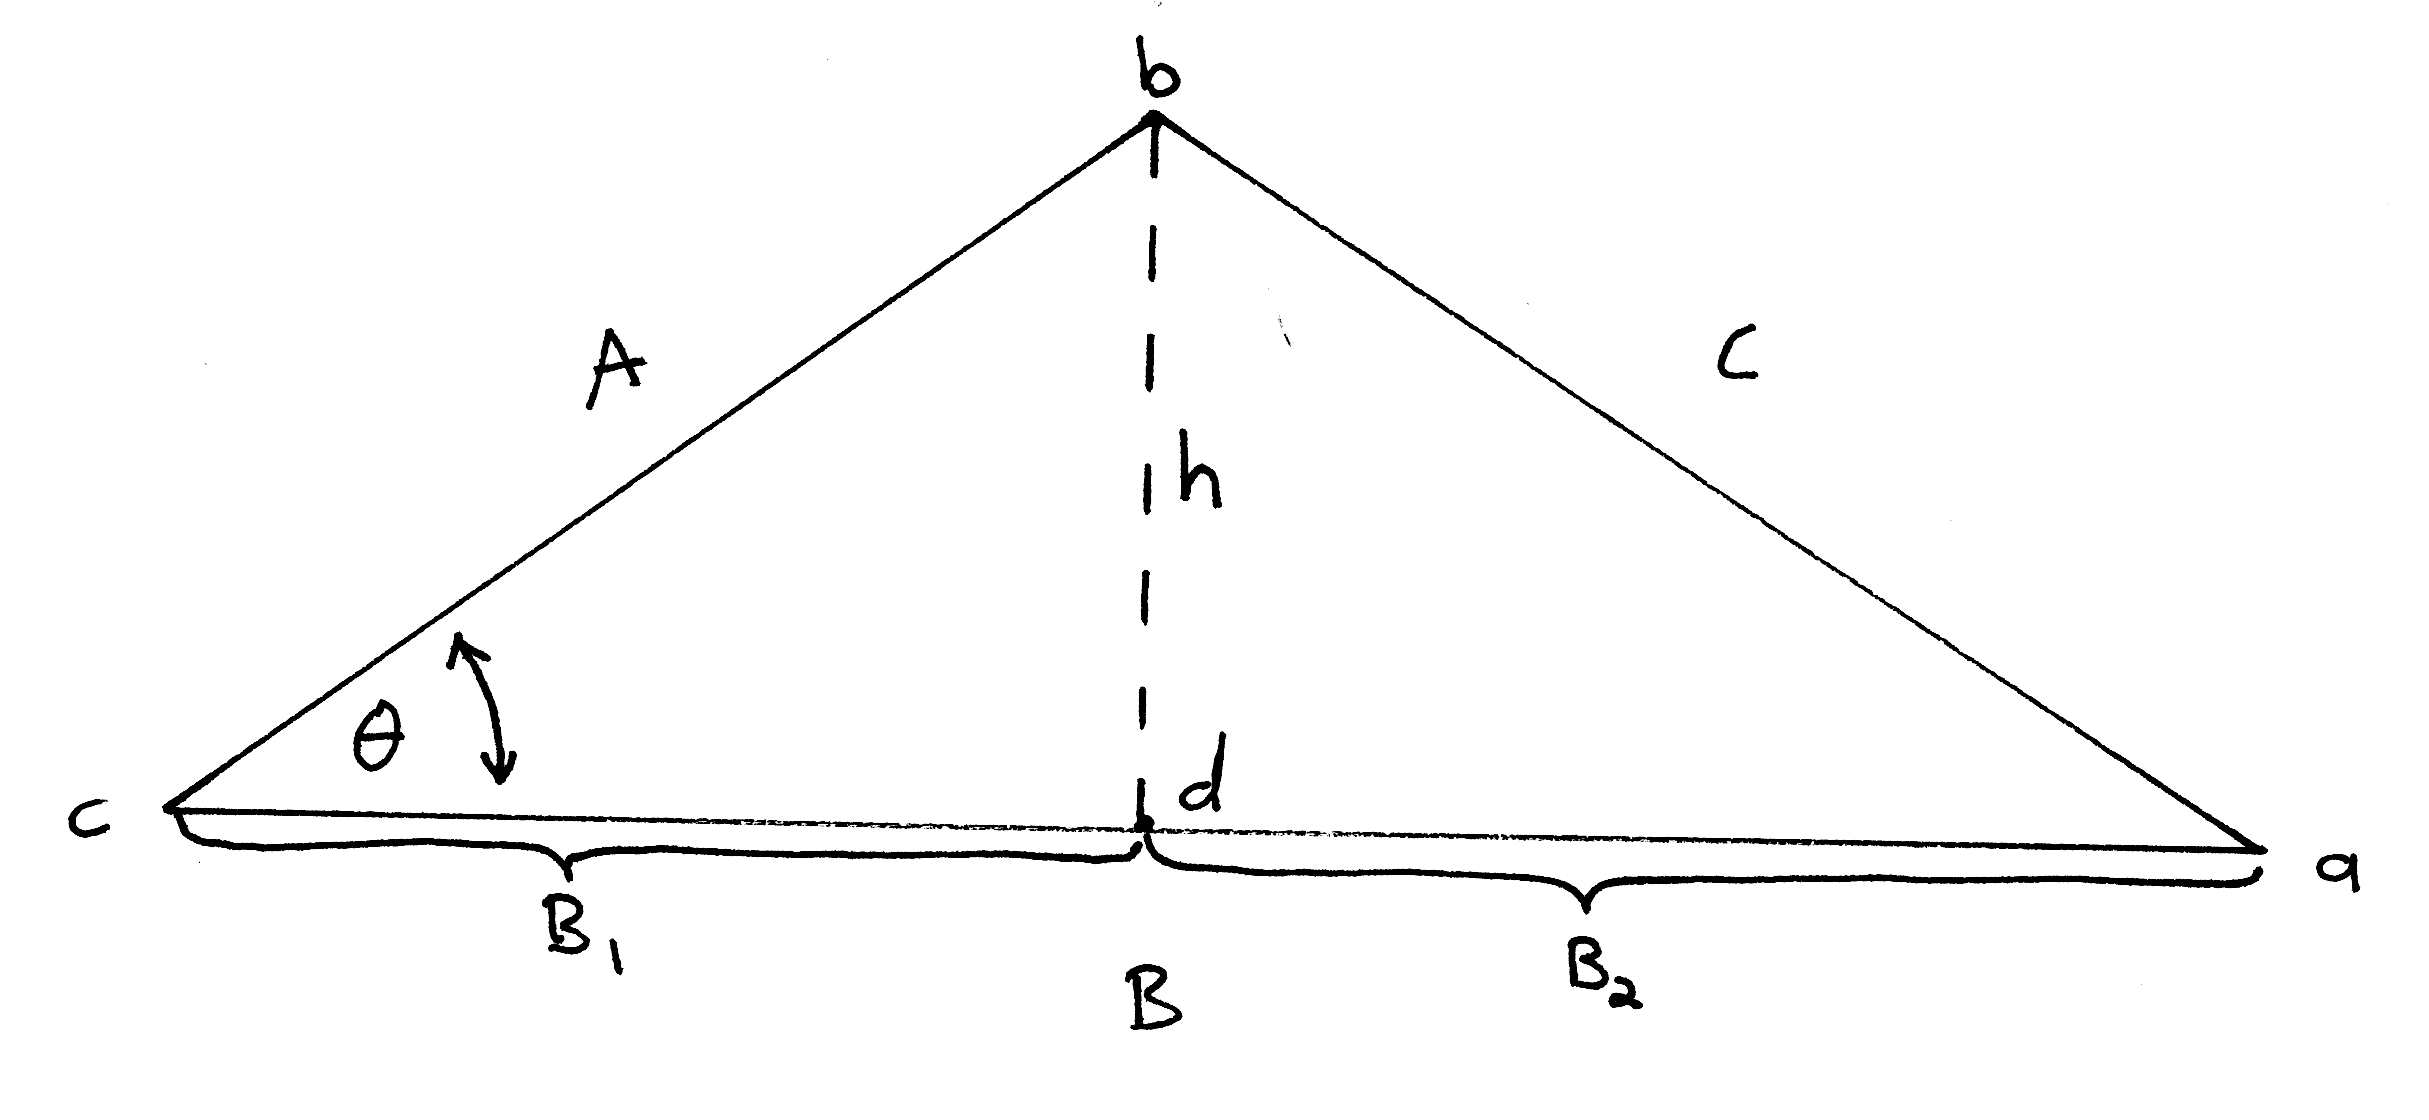
\includegraphics[width=2.5in]{images/lawofcosB.jpg}

\caption{Law of Cosines: $C^2 = A^2 + B^2 - 2AB \cos(\theta)$  \label{fig:lawofcos}}
\end{figure}

Let $\triangle abc$ be a general triangle as in Figure \ref{fig:lawofcos}
and let $\theta$ be the angle $\angle bca$.
Let $A,B,C$ be the the lengths of the edges opposite the angles $a,b,c$ respectively,
as shown in the following figure:

The Law of Cosines states that the following relationship holds for any such triangle:
\[
C^2 = A^2 + B^2 - 2AB\cos(\theta)
\]
To prove this relation, we decompose the triangle $\triangle abc$ into two right triangles
$\triangle adb$ and $\triangle cdb$ and let $h$ be the length of the common side $bd$
and $B_1$ and $B_2$ the lengths $cd$ and $da$ respectively. Then, by the definition of
the cosine we know that
\[
B_1 = A*\cos(\theta)
\]
and from the Pythagorean Theorem we know that
\begin{eqnarray*}
A^2 &=& B_1^2 + h^2 \\
C^2 &=& B_2^2 + h^2
\end{eqnarray*}
and since $B = B_1 + B_2$ we see that
\begin{eqnarray*}
B^2 &=& (B_1+B_2)^2 \\
&=& B_1^2 + 2B_1B_2 + B_2^2
\end{eqnarray*}
So
\begin{eqnarray*}
C^2-(A^2 + B^2) &=& B_2^2 + h^2  - (B_1^2 + h^2 + B_1^2 + 2B_1B_2 + B_2^2) \\
&=& B_2^2 + h^2  - B_1^2 - h^2 - B_1^2 - 2B_1B_2 - B_2^2 \\
&=&  -2 B_1^2 - 2B_1B_2  \\
&=&  -2 B_1(B_1+B_2) \\
&=&  -2 B_1 B \\
&=&  -2 (A \cos(\theta)) B \\
&=&  -2 A  B \cos(\theta)
\end{eqnarray*}
and so
\[
C^2 = A^2 + B^2 - 2 A B \cos(\theta)
\]

To apply the law of cosines to the dot product, observe that if  $\vect {u} $ and $\vect{v}$
are two vectors then the three points $\vect{u}$, $\vect{v}$, and the origin $\vect{o}$ all
lie in a plane and form a triangle in that plane. We can let $A$ be the length of $\vect{u}$ and
$B$ be the length of $\vect{v}$  and let $C$ be the length of the third side $\vect{w}=\vect{v}-\vect{u}$
and let $\theta$ be the angle between $\vect{u}$ and $\vect{v}$.

By the Law of Cosines we know that:
\[
C^2 = A^2 + B^2 - 2AB \cos(\theta)
\]
and since $A^2=\vect{u}\cdot\vect{u}$, $B^2=\vect{v}\cdot \vect{v}$, $C^2=\vect{w}\cdot \vect{w}$ we have
\[
\vect{w}\cdot\vect{w} = \vect{u} \cdot \vect{u} + \vect{v} \cdot \vect{v} - 2 A B \cos(\theta)
\]
Substituting in $\vect{w} = \vect{v} - \vect{u}$  and using the distributive property of the dot product
we find that
\begin{eqnarray*}
\vect{u} \cdot \vect{u} + \vect{v} \cdot \vect{v} - 2 A B \cos(\theta) &=&
\vect{w}\cdot\vect{w}  \\
&=&  (\vect{v} - \vect{u}) \cdot (\vect{v} - \vect{u}) \\
&=&  \vect{v}\cdot \vect{v} -  \vect{u}\cdot \vect{v} -  \vect{v}\cdot \vect{u}  + \vect{u}\cdot \vect{u}
\end{eqnarray*}
and so
\begin{eqnarray*}
 - 2 A B \cos(\theta) &=&
 - 2 \vect{u}\cdot \vect{v} \\
\end{eqnarray*}
from which the dot product property follows immediately from $A = \vert \vect{u}\vert$ and
$B = \vert \vect{v}\vert$:
\begin{eqnarray*}
 \vect{u}\cdot \vect{v} &=&  \vert \vect{u}\vert\; \vert \vect{v} \vert \; \cos(\theta)
\end{eqnarray*}

\subsection{Dot Product as Matrix Multiplication}
If we think of $\vect p$ and $\vect q$ as being column matrices
\[
p = \left (\begin{array}{c} p_x \\ p_y \\ p_z \end{array} \right )
\;\;\;
q = \left (\begin{array}{c} q_x \\ q_y \\ q_z \end{array} \right )
\]
then we can also write the dot product as a matrix multiplication of a (1x3) and a (3x1) matrix
to get a 1x1 matrix:
\[
p\cdot q = p^T*q = (p_x\; p_y \;p_z)*
\left (\begin{array}{c} q_x \\ q_y \\ q_z \end{array} \right )
=p_xq_x + p_yq_y + p_zq_z
\]
and where $M^T$ denotes the transpose of the matrix $M$, that is the matrix
whose rows and columns are reversed:
\[
M^T_{i,j} = M_{j,i}
\]


\section{The Cross Product}
The cross product is a very useful operation which allows one to take any two
vectors $\vect u$ and $\vect v$ and to generate a new vector $\vect u \times \vect v$
called the cross product of $\vect u$ and $\vect v$ which has the property that it is
perpendicular to both $u$ and $v$. Equivalently, if $u$ and $v$ are not multiples of each other,
then they define a 2d plane in 3D space, and their cross product $\vect u \times \vect v$ will be perpendicular to that plane.

The cross product is relatively easy to compute using the following formula:
\[
\vect u \times \vect v = (u_yv_z-u_zv_y, u_zv_x-u_xv_z, u_xv_y-u_yv_x) \\
\]
and it satisfies the following properties:
\[
(\vect u \times \vect v) \cdot u = 0 \;\;
(\vect u \times \vect v) \cdot v = 0
\]

\subsection{Proof that the cross product $\vect u \times \vect v$ is perpendicular to $\vect u$ and $\vect v$}
To prove this we need some linear algebra. Lets assume that $\vect u$ and $\vect v$ do not lie on the same line
in 3D space, then they must be linearly independent and hence they uniquely define a 2d plane $P$. Recall that if
$\vect w$ is any vector, then $\vect w$ lies in the plane defined by $\vect u$ and $\vect v$ if and only if
the determinant with rows $\vect u$, $\vect v$, and $\vect w$ is zero, that is
\[
\begin{array}{|ccc|}
u_x & u_y & u_z \\
v_x & v_y & v_z \\
w_x & w_y & w_z
\end{array}
= 0
\]
We can compute the determinant by expanding the minors along the bottom row to get
\begin{eqnarray*}
\begin{array}{|ccc|}
u_x & u_y & u_z \\
v_x & v_y & v_z \\
w_x & w_y & w_z
\end{array}
&=& w_x(u_yv_z - u_zv_y) - w_y(u_xv_z - u_zv_x) + w_z(u_xv_y - u_yv_x) \\
&=& (w_x,w_y,w_z) \cdot (u_yv_z - u_zv_y, -(u_xv_z - u_zv_x) , u_xv_y - u_yv_x) \\
&=& \vect w \cdot (\vect u \times \vect v)
\end{eqnarray*}
Thus, we see that for any vector $w$ and for any two non-collinear vectors $u$ and $v$, we have $\vect w \cdot (\vect u \times \vect v) $ is zero if and only if $w$ is in the same
plane $P$ as $u$ and $v$, and so we conclude that
\[
\vect u \cdot (\vect u \times \vect v) = 0 \;\;
\vect v \cdot (\vect u \times \vect v) = 0
\]
\subsection{The Matrix representation of cross product}
The cross product  $\vect u \times \vect v$ can also be represented using matrix multiplication.
Indeed, let $u^\flat$ denote the following matrix constructed from a vector $u$:
\[
u^\flat =
\left (
\begin{array}{ccc}
0& -u_z & u_y \\
u_z& 0 & -u_x \\
-u_y & u_x & 0 \\
\end{array}
\right )
\]
and observe that $(\vect u \times \vect v) = \vect u ^ \flat * \vect v$


\section{Representing rays as a function of time}
A ray is represented by an origin vector $\vect p = (p_x, p_y, p_z)$
and a direction vector $\vect d = (d_x,d_y,d_z)$. The parametric form
of a ray is shown below.
\[
{\vect r} (t) = {\vect p} + t*{\vect d}
\]
It is a function of a single variable $t$
and can be thought of as returning the position ${\vect r} (t)$ of a point
that starts at the origin ${\vect p}$ and moves in direction ${\vect d}$
at a constant rate of $\vert \vect d \vert $ units per time unit.
We will usually assume that the direction $d$ of a ray has length 1.

Equivalently, we can compute the component functions for ${\vect r}$
\[
{\vect r} (t) = (r_x(t), r_y(t), r_z(t))
\]
\begin{eqnarray*}
r_x(t) &=& p_x + t*d_x  \\
r_y(t) &=& p_y + t*d_y  \\
r_z(t) &=& p_z + t*d_z
\end{eqnarray*}


When tracing rays, we think of light particles moving out along the ray until they hit an
object (which is of course the reverse of what actually happens!). The method {\tt r.atTime(t)}
returns the point on the ray whose distance from the origin is given by ${ t*\vert \vect d \vert}$. If we
think of the light moving along the ray at a speed of $\vert \vect d \vert$ units per second, then {\tt r.atTime(t)}
returns the location after {\tt t} seconds.



\section{Representing Vectors and Rays in Javascript}
Fig.~\ref{fig:Vector3class} shows a Javascript class Vector3 representing 3d vectors and Fig.~\ref{fig:Ray3class}
shows an implementation of Rays, which consist of a point vector $p$ and a direction vector $d$.
We will use vectors and points interchangeably.

The Vector3 class implements the operations to add, subtract, and scale a vector as well as the dot and cross product operators. These are available both as static methods and as instance methods. For example, here is some code to create two vectors
\begin{verbatim}
const v = new Vector3(1,2,2)
const w = new Vector3(-2,2,-1)
console.log("v.w = "+v.dot(w))
\end{verbatim}
The Ray3 class provides a constructor {\tt new Ray3(p,d)} and an atTime(t) method which shows the position of a point that starts at position $p$ and moves with velocity $d$ for $t$ units of time.


\section{Exercises  \label{ex:vectors}}
Consider the following four points
\begin{eqnarray*}
a &=& (1, 2, 2) \\
b &=& (7, -2, 4) \\
c &=& (0, 4, -2) \\
d &=& (1, 1, 1)
\end{eqnarray*}
Let $u$ be the vector from b to a, and let $v$ be the vector from b to c.
Let $P$ be the plane that passes through $d$ and is normal to $a$.
\begin{enumerate}
\item How long is the vector $u$?
\item Is the angle between u and v less than 90 degrees, equal to 90 degrees, or greater than 90 degrees? How do you know?
\item Calculate the normalization of the vector $a$, i.e. the unit vector pointing in the same direction as $a$.
\item How far away is the point $b$ from the plane $P$?
\item Find the point $p$ which is the projection of $b$ onto the plane $P$.
\item Use the cross product to find a vector $w$ which is perpendicular to $u$ and $v$.
\item Find the point $e$ that you get by rotating the point $c$ around the $x$ axis by 90 degrees.
\end{enumerate}






\begin{figure}
\begin{verbatim}
class Vector3 {
  // this is the class of 3 dimensional vectors

  constructor(x,y,z){
    this.x=x; this.y=y; this.z=z;
  }

  static dot(u,v) {
    return u.x*v.x + u.y*v.y + u.z*v.z
  }
  static add(u,v){
    return new Vector3(u.x+v.x, u.y+v.y, u.z+v.z)
  }
  static subtract(u,v){
    return new Vector3(u.x-v.x, u.y-v.y, u.z-v.z)
  }
  static scale(u,k){
    return new Vector3(u.x*k, u.y*k, u.z*k)
  }
  static cross(u,v){
    return new Vector3(u.y*v.z-u.z*v.y, u.z*v.x-u.x*v.z, u.x*v.y-u.y*v.x)
  }

  dot(v){
    return Vector3.dot(this,v)
  }
  cross(v){
    return Vector3.cross(this,v)
  }
  add(v){
    return Vector3.add(this,v)
  }
  subtract(v){
    return Vector3.subtract(this,v)
  }
  scale(k){
    return Vector3.scale(this,k)
  }

  length(){
    return Math.sqrt(this.dot(this))
  }
  normalize(){
    return this.scale(1/this.length())
  }

  toString(){
    return "Vector3("+this.x+","+this.y+","+this.z+")";
  }

}
\end{verbatim}
\caption{Vector3 class\label{fig:Vector3class}}
\end{figure}

\begin{figure}
\begin{verbatim}
class Ray3 {
  constructor(p,d){
    // s and d are Vector3 objects
    // this represents a ray starting at s moving in direction d
    this.p = p
    this.d = d
    this.len = d.length()
  }

  atTime(t){
    return this.p.add(this.d.scale(t))
  }

  toString(){
    return "Ray3("+this.p+","+this.d+")";
  }


}
\end{verbatim}
\caption{Ray3 class\label{fig:Ray3class}}
\end{figure}




\chapter{Basic Ray Tracing}


In this chapter we develop the fundamental ray tracing algorithms and ask you to provide an implementation for the corresponding objects. The main algorithm is the following:
\begin{verbatim}
for each pixel p to be displayed on the canvas
    use the camera object to create the ray r corresponding to that pixel
    find the closest intersection k of that ray with any object in the scene
    use the information about that intersection to determine the color for that pixel
    draw that color on the canvas
\end{verbatim}
In this chapter we show how to implement this algorithm to draw spheres of various sizes and locations in a scene containing a number of lights at various positions.  All raytracing will be done in monochrome (shades of gray). The goal is to get a minimal ray tracer implemented as quickly as possible. In the rest of this Chapter we talk about the various classes you will need to implement as well as the key algorithms you will need to code up.

\section{Renderers, Cameras, and Scenes}
We will follow the ThreeJS model of rendering a scene by creating a renderer, a camera, and a scene and asking the renderer to draw a view of the scene from the specified camera. The standard code for generating a view will be
to first create a renderer by specifying the dimension of its virtual screen. The renderer will draw on the HTML div element with id 'canvas' and it will draw an image with the specified resolution:
\begin{verbatim}
const renderer = new Renderer(300,300)
\end{verbatim}
Next, we create a camera, which by default sits at the origin (0,0,0) looking down the z axis. We can translate it in the z-direction. Later we will see how to position it anywhere.
\begin{verbatim}
const camera = new Camera()
camera.translateZ(10)
\end{verbatim}
Finally we create a Scene and we give it a name
\begin{verbatim}
const scene = new Scene("main")
\end{verbatim}
Assuming we have added objects to the scene (as described in the next section). We can draw the scene on the canvas with the command:
\begin{verbatim}
renderer.render(scene.camera)
\end{verbatim}
just as with ThreeJS.

The code for our Renderer, Camera, and Scene classes is in Figs.~\ref{fig:RendererClass},\ref{fig:CameraClass},\ref{fig:SceneClass} 
The three most complex methods in these classes are
\begin{verbatim}
renderer.render(scene,camera)
camera.createRay(x,y)
scene.intersect(ray)
\end{verbatim}
The renderer.render method loops through each of the virtual pixels (i,j) and uses them to
create a point in the (x,y) square from [-1,1]x[-1,1]. It then uses that point to create a ray r
and then intersects that ray with the scene to get an intersection object.
If the intersection is empty, then it draws the background color, otherwise it finds the color of the object at that point.

The camera.createRay(x,y) simply creates a ray starting a the camera position and looking down the z axis but offset by the (x,y) values.

The scene.intersect(ray) method intersects the ray with every object in the scene
Then filters out the ones that have empty intersections, and finally loops through that list of intersections to find the closest one.  Each RayIntersection object contains the object the ray hit, the intersection point, and the distance
\begin{figure}
\begin{verbatim}
class Renderer {
  constructor(w,h){
    this.width = w
    this.height = h
  }

  drawPixel(i,j,c){
    var canvas = document.getElementById('canvas');
    if (canvas.getContext) {
      var ctx = canvas.getContext('2d')
      ctx.fillStyle = c;
      var w = canvas.width
      var h = canvas.height
      var wp = w/this.width
      var hp = h/this.height
      ctx.fillRect(i*wp,(this.height-j-1)*hp,wp,hp);
    }
  }

  render(scene,camera){
    for(let i=0;i<this.width;i++){
      for(let j=0; j<this.height; j++){
        const x = 2*i/this.width-1 // x goes from -1 to 1 in this.width steps
        const y = 2*j/this.height-1 // y goes from -1 to 1 in this.height steps
        const r = camera.createRay(x,y) // this creates the ray for pixel (i,j)
        const intersection = scene.intersect(r)
        if (intersection.isEmpty()){
          this.drawPixel(i,j,'rgb(0,0,0)')
        }
        else {
          const obj = intersection.object
          const p = intersection.point
          const c = obj.color(p)
          this.drawPixel(i,j,c)
        }
      }
    }
  }
}
\end{verbatim}
\caption{\label{fig:RendererClass}}
\end{figure}

\begin{figure}
\begin{verbatim}
class Camera {
  constructor(){
    this.position = new Vector3(0,0,0);
  }

  translateZ(k){
    this.position.z += k
  }

  createRay(x,y){
    // this creates a ray looking in the negative z direction
    var p = this.position;
    var d = new Vector3(x,y,-1)
    var r = new Ray3(p,d);
    return r;
  }
}
\end{verbatim}
\caption{\label{fig:CameraClass}}
\end{figure}

\begin{figure}
\begin{verbatim}

class Scene {
  constructor(name){
    this.name=name
    this.objects=[]
    this.lights=[]
  }

  addObject(x){
    this.objects.push(x)
  }

  addLight(x){
    this.lights.push(x)
  }

  intersect(ray){
    // intersect the ray with each object
    let z = this.objects.map(
      function(x){
        return x.intersect(ray)});
    //console.dir(z)
    // throw out the non-intersections
    z = z.filter(
      function(x){
        return x.object!= null})
    //console.dir(z)
    // if the ray didn't intersect any objects, return a non-intersection object
    if (z.length==0)
      return RayIntersection.none()

    // now we know it did intersect an object so lets find the closest one
    let mindist=z[0].distance
    let minIntersection=z[0]
    for(let x of z){
      if (x.distance < mindist) {
        mindist = x.distance
        minIntersection = x
      }
    }
    return minIntersection

  }
}
\end{verbatim}
\caption{\label{fig:SceneClass}}
\end{figure}

\newpage 
\section{Finding the intersection of a ray and a sphere}
Next we show how to implement the rayIntersect method for a sphere.
This will allow you to create your first raytracer which projects the objects
in a scene onto the canvas and uses the distance of the intersection point from the
camera to choose the color for the pixel.  In the next Chapter we'll look at how to
implement lighting models in the Ray Tracer.

In this section, we show how to compute the intersection of a ray and a sphere
using the 3D coordinates directly. In the next section, we provide a simpler
approach using vector algebra, and this will be the approach we use with all later
objects.

\subsection{Representing spheres}


A sphere $S_{{\vect c},r}$ consists of all 3D points $q$ which are a constant distance $r$
from the center ${\vect c} = (c_x,c_y,c_z)$ of the sphere. The equation
that determines whether a point $q=(x,y,z)$ is on the sphere of radius
$r$ and center ${\vect c}$ is
\[
(x-c_x)^2 + (y-c_y)^2 + (z-c_z)^2 = r^2
\]
This is an implicit representation of the sphere and can be thought of as
a test of whether a point is on the sphere.

\subsection{Intersecting a ray with a sphere}
Let  $\vect R(t) = (R_x(t), R_y(t),R_z(t))$  be the ray that starts at position $\vect p=(p_x,p_y,p_z)$
and points out in direction $\vect d=(d_x,d_y,d_z)$
To determine the intersection of the ray $\vect R$
with a sphere $S_{{\vect c},r}$, we proceed as follows:
\begin{eqnarray*}
 r^2  &=& (R_x(t)-c_x)^2 + (R_y(t)-c_y)^2 + (R_z(t) - c_z)^2\\
 &=&
   (d_x t + p_x - c_x)^2 + (d_y t + p_y - c_y)^2 + (d_z t + p_z - c_z)^2  \\
 &=& d_x^2 t^2 + 2 d_x t (p_x-c_x) + (p_x-c_x)^2 \\
&& + d_y^2 t^2 + 2 d_y t (p_y-c_y) + (p_y-c_y)^2 \\
&& + d_z^2 t^2 + 2 d_z t (p_z-c_z) + (p_z-c_z)^2
\end{eqnarray*}
So, grouping the terms by powers of $t$ we find that ${\vect R}(t)$ is on
the sphere if and only if
\[
A t^2 + B t + C = 0
\]
where
\begin{eqnarray*}
A &=& d_x^2 + d_y^2 + d_z^2 \\
B &=& 2 (d_x(p_x-c_x) + d_y(p_y-c_y) + d_z(p_z-c_z)) \\
C &=& (p_x-c_x)^2 + (p_y-c_y)^2 + (p_z-c_z)^2 - r^2
\end{eqnarray*}
and we can solve this using the quadratic equation. We do this
by first evaluating the discriminant $D = B^2 - 4 A C$.

If $D < 0$ then there are no solutions, so the ray does not intersect
the Sphere.

If $D = 0$, then there is one solution $T = -B/(2A)$ and if this is
positive, then the ray intersects the sphere
at exactly one point and does not pierce the interior of the sphere

If $D > 0$ then there are two solutions $t_1 < t_2$
\begin{eqnarray*}
t_1 &=& (-B - sqrt(D))/(2A)  \\
t_2 &=& (-B + sqrt(D))/(2A)  \\
\end{eqnarray*}
If both are negative, then the ray does not intersect the sphere.
If one is negative and one is positive, the starting point {\vect p} of the ray is inside the Sphere
and it intersects the sphere going forward at time $t_2$ and going backward at time $-t_1$. If both are positive, then the starting point of the ray
is outside the sphere and intersects it for the first time at time $t_1$.

\subsection{Corner cases}
We've left a few tricky cases out of the analysis above. For example,
suppose the discriminant $D$ is positive, so there are two solutions.
What does it mean if one of them is zero? Also, what does it mean if
the two intersection points $t_1$ and $t_2$ are very close (say less than
0.000000001 units apart?) We will need to deal with these ``corner cases''
in any practical ray tracer we write.

\subsection{Finding the intersection point}
Once we have found the ``time'' $t_0$
of the earliest intersection of the ray
with the sphere, we can find the intersection point by evaluating
${\vect R}$
at that time.
\begin{eqnarray*}
{\vect R}(t_0) &=& (R_x(t_0), R_y(t_0),R_z(t_0)) \\
&=&
(p_x + t_0*d_x, p_y + t_0*d_y, p_z + t_0*d_z)
\end{eqnarray*}



\section{RayTracing a sphere using vector notation}
Now we reproduce the same derivations as in the previous section, but using
vector algebra instead. You will see that the calculations are considerably
simpler.

A sphere consists of all 3D points which are a constant distance $r$
from the center of the sphere ${\vect c} = (c_x,c_y,c_z)$. The equation
that determines whether a point ${\vect v}$ is on the sphere of radius
$r$ and center ${\vect c}$ is
\[
\vert {\vect v} - {\vect c} \vert = r
\]
This is an implicit representation of the sphere and can be thought of as
a test of whether a point is on the sphere.

\subsection{Intersecting a ray with a sphere in vector notation}
To determine the intersection of a ray $\vect R(t) = {\vect p} + t {\vect d}$
with a sphere $S_{{\vect c},r}$. We look for points ${\vect v}$ on the
Sphere which are also on the ray, and hence have the form: $\vect v = {\vect p} + t {\vect d}$
\begin{eqnarray*}
r^2 &=& \vert {\vect v} - {\vect c} \vert^2 \\
 &=& ({\vect v} - {\vect c}) \cdot ({\vect v} - {\vect c}) \\
 &=& (t {\vect d} + {\vect p} - {\vect c}) \cdot (t {\vect d} + {\vect p} - {\vect c}) \\
 &=& \vert {\vect d} \vert^2 t^2 + 2 {\vect d} \cdot({\vect p} - {\vect c}) t + \vert {\vect p} - {\vect c}\vert^2
\end{eqnarray*}
So, grouping the terms by powers of $t$ we find that ${\vect r}(t)$ is on
the sphere if and only if
\[
A t^2 + B t + C = 0
\]
where
\begin{eqnarray*}
A &=& \vert {\vect d} \vert^2  \\
B &=&  2 {\vect d} \cdot({\vect p} - {\vect c})  \\
C &=& \vert {\vect p} - {\vect c}\vert^2 - r^2
\end{eqnarray*}
and we can solve this using the quadratic equation {\bf {exactly}} as we did before.

{\it
We do this by first evaluating the discriminant $D = B^2 - 4 A C$.

If $D < 0$ then there are no solutions, so the ray does not intersect
the Sphere.

If $D = 0$, then there is one solution $T = -B/(2A)$ and if this is
positive, then the ray intersects the sphere with a glancing blow
at exactly one point and does not pierce the interior of the sphere.

If $D > 0$ then there are two solutions $t_1 < t_2$
\begin{eqnarray*}
t_1 &=& (-B - sqrt(D))/(2A)  \\
t_2 &=& (-B + sqrt(D))/(2A)  \\
\end{eqnarray*}
If both are negative, then the ray does not intersect the sphere.
If one is negative and one is positive, the ray is inside the Sphere
and it intersects the sphere at time $t_2$. If both are positive, then
it is outside the sphere and intersects it at time $t_1$.
}

\section{The Sphere and RayIntersect classes}
We can encapsulate the algorithms of the previous section into the Sphere
class, which represents a sphere and provides methods for intersecting
a ray with a sphere (and in the process finding the distance from the origin
of the ray to the sphere).

The code for storing a RayIntersection element is in 
Figure \ref{fig:RayIntersectionClass}, and the code for the Sphere object is in
Figure \ref{fig:SphereClass}.  At this point we are generating a colors for points on the Sphere in terms of their coordinates. In the next chapter we will look at lighting models and generate realistic lighting effects.





Given this code, we can now render a scene with two spheres
with the following code.
\begin{verbatim}
function runTest(){
        canvas.width=900
        canvas.height=900
        const renderer = new Renderer(900,900)
        const scene = new Scene('demo0')
        const camera = new Camera()
        camera.translateZ(10)
        const s1 = new Sphere(new Vector3(-2,0,-8),2)
        scene.addObject(s1)
        const s2 = new Sphere(new Vector3(2,0,-9),3)
        scene.addObject(s2)
        renderer.render(scene,camera)
}

runTest()
\end{verbatim}



\begin{figure}
\begin{verbatim}
class RayIntersection{
  constructor(object, point, distance){
    this.object=object
    this.point = point
    this.distance=distance
  }

  static none(){
    return new RayIntersection(null, null, -1);
  }

  isEmpty(){
    return this.object==null
  }
}
\end{verbatim}
\caption{RayIntersect \label{fig:RayIntersectClass}}
\end{figure}



\begin{figure}
\begin{verbatim}

class Sphere {
  constructor(c,r){
    this.center = c
    this.radius = r
  }

  intersect(r){
    // intersect the ray r with the sphere
    const a = (r.d).dot(r.d)
    const pc = r.p.subtract(this.center)
    const b = 2*(r.d.dot(pc))
    const c = pc.dot(pc) - this.radius*this.radius
    const d = b*b-4*a*c
    if (d<0) return []
    const t1 = (-b - Math.sqrt(d))/(2*a)
    const t2 = (-b + Math.sqrt(d))/(2*a)
    const p1 = r.atTime(t1);
    const p2 = r.atTime(t2);

    if (d==0)
       if (t1>0)
        return new RayIntersection(this,p1,p1.subtract(r.p).length())
      else
        return RayIntersection.none()

    if (t1>0)
      return new RayIntersection(this,p1,p1.subtract(r.p).length())
    else if (t2>0)
      return new RayIntersection(this,p2,p2.subtract(r.p).length())
    else
      return RayIntersection.none()
  }



  color(p){
    // return the color of a the point p on the Sphere
    // this ignore lights and just uses the position of the point on the sphere
    // First we rescale the point so that its x,y,z values range from 0 to 256
    const q = p.subtract(this.center).scale(128/this.radius).add(new Vector3(128,128,128))
    //Then we use those values to create a color
    const c =  'rgb('+Math.floor(q.x)+','+Math.floor(q.y)+','+Math.floor(q.z)+')'
    //console.log(c)
    return(c)
  }

}

\end{verbatim}
\caption{Sphere \label{fig:SphereClass}}
\end{figure}










\chapter{Lighting Models}
In the previous chapters we developed several classes representing 3D objects.
In this chapter we add lights to the program and introduce the three main lighting
effects used in 3D graphics engines: ambient, diffuse, and specular illumination.

\section{Materials}
For this initial version of the ray tracer, we introduce a {\tt Material} object which will store two properties.
\begin{itemize}
\item the color of the object (which will be a number ranging from 0.0 for black to 1.0 for white).
\item the shininess of the object which is a number ranging from not shiny (0) to very shiny (typically 511=$2^9-1$)
\end{itemize}
We will need to modify the color method of the sphere class (and any other objects we create) so that it uses this lighting model.

One might also want to specify two different materials: one for the outside of the object and the other for the inside. The outside material describes the surface of the object when seen from outside. The inside material describes how it looks from inside. We could imagine sphere which is a mirror on the outside but a flat matte blue on the inside. If the camera is positioned inside the sphere, a particular point on the sphere will look much different than if it is viewed from outside the sphere!

\section{Ambient illumination}
The ambient lighting model assigns a fixed intensity of light to any visible part
of an object. This ambient intensity does not depend on the presence of any lights
in the scene. It models the general light that bounces off the walls of a room
and fills the space uniformly with a low level of light. Ambient light is handled
in two places. First, it is a parameter of the scene and provides a light level
that is used to illuminate all objects in the scene. Second, each light has an
ambient parameter, which provides a low level of light for any objects that are
visible to the light.

\section{Diffuse illumination}
Diffuse illumination models light that hits a rough surface and is scattered
equally in all directions. The intensity of the light depends on the angle
at which the light hits the surface. Thus light directly overhead will
maximize the diffuse illumination whereas light coming from a point just over the
horizon will be very weak.

More precisely, the model is that the diffuse lighting at a point
is directly proportional to how much that light is spread out on the surface. When shining straight down (at high noon) the diffuse lighting is brightest, when coming in from near 90 degrees (e.g. sunset), the diffuse lighting is nearly zero.
In Figure \ref{fig:diffuse} we see a beam of light of width $\epsilon$ hitting a plane at an angle of $\beta$ from the plane and $\alpha$ from the vertical. This illuminates a region of length $\delta$.  The diffuse illumination at any point in that region is defined to be $\epsilon/\delta$.  So if the light was shining straight down (i.e. $\alpha=0$) then the diffuse illumination would be 1, whereas if it is parallel to the plane then the diffuse illumination would be zero.

\begin{figure}[h]
\centering
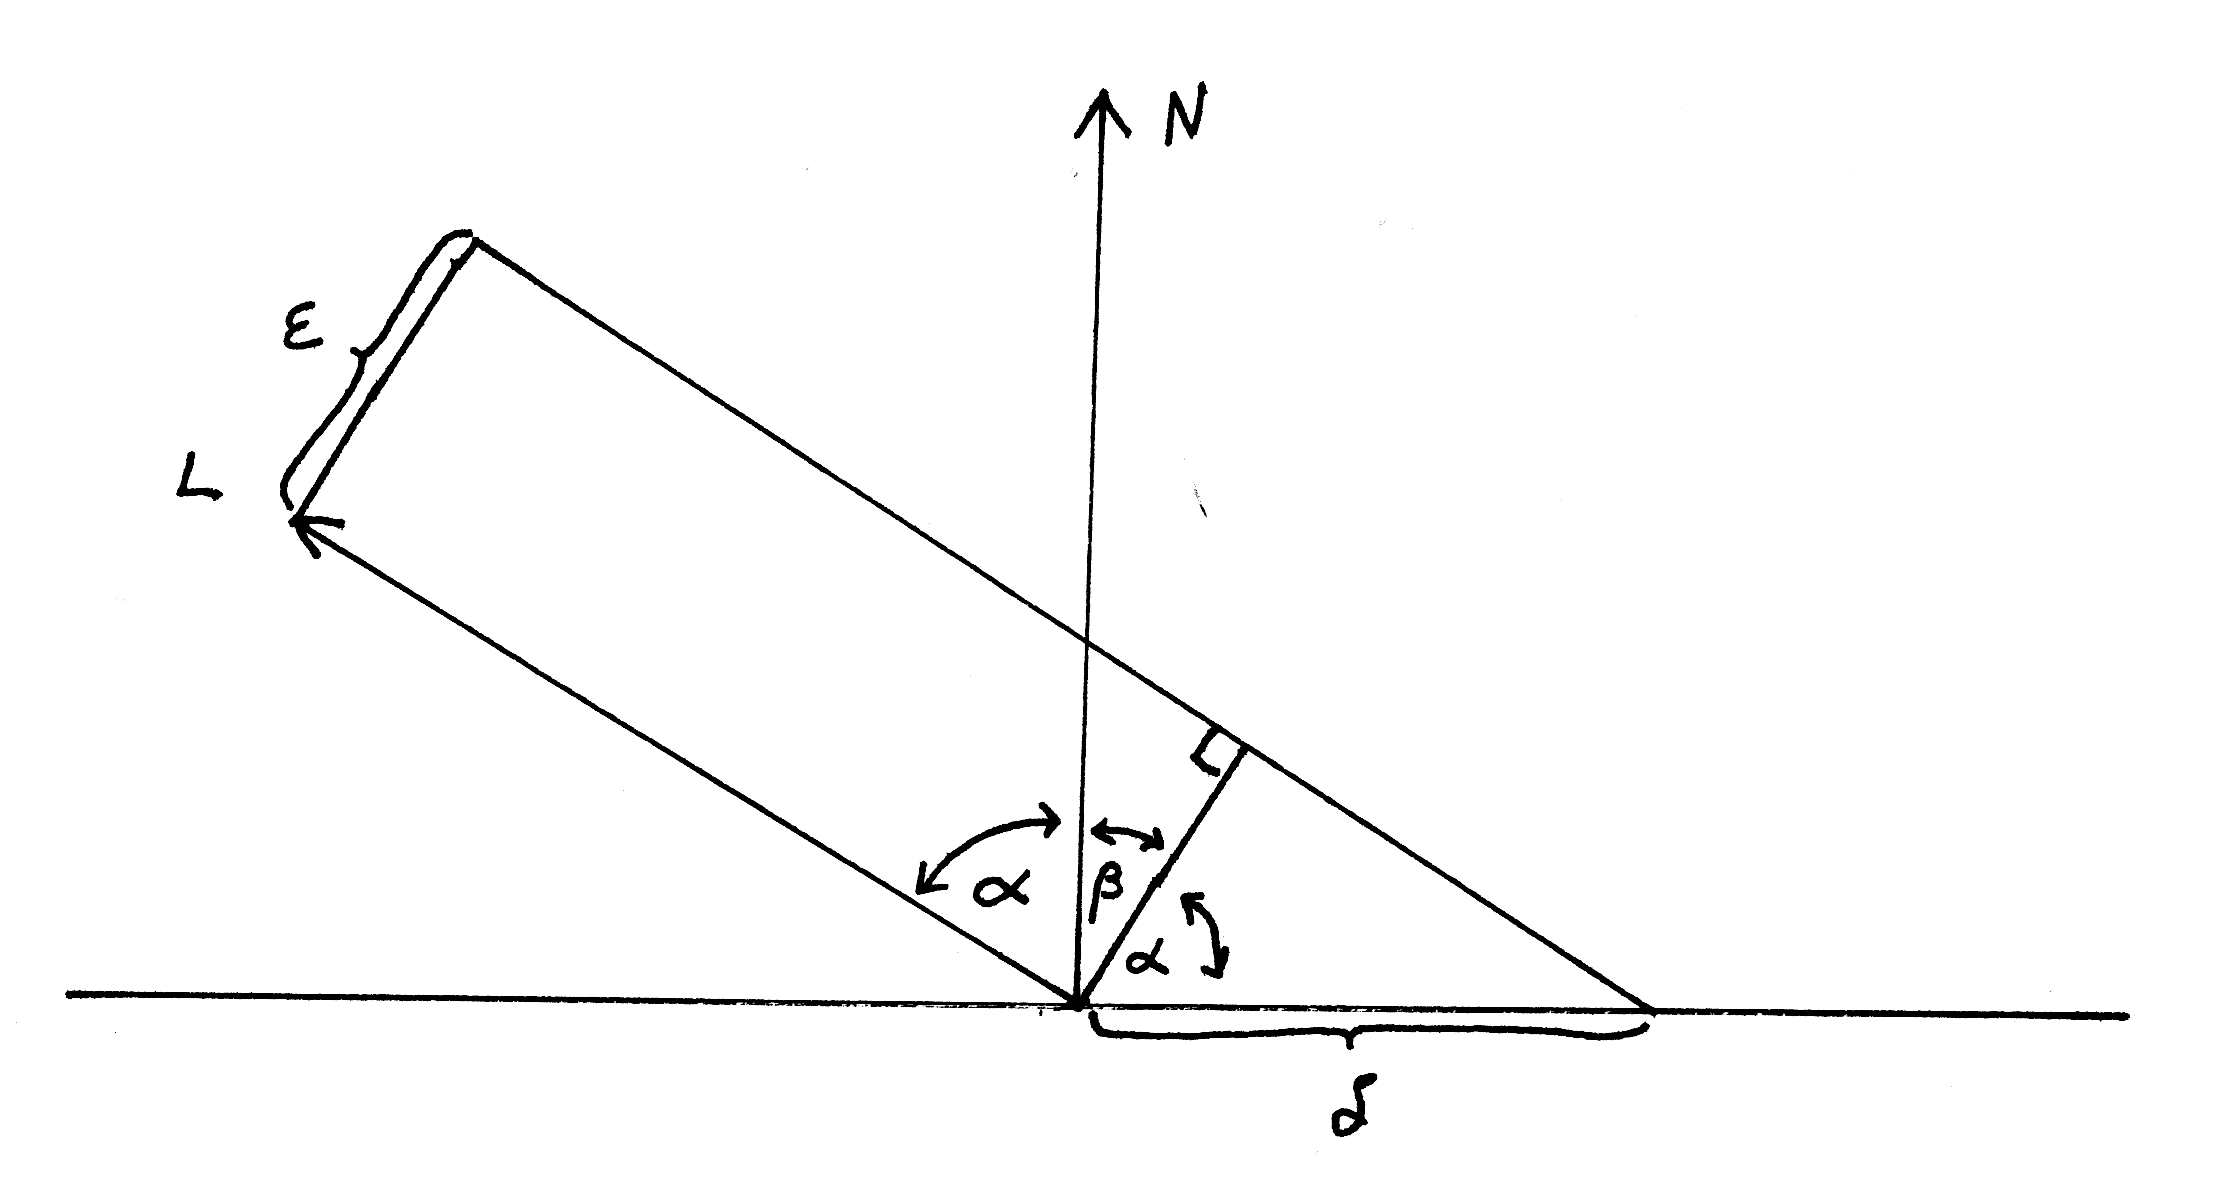
\includegraphics[width=2.5in]{images/diffuse2.jpg}
\caption{Diffuse illumination is smaller when one unit of light is spread over a larger region\label{fig:diffuse}}
\end{figure}

With a little geometry, we can see that $\epsilon/\delta = cos(\alpha)$ which in turn can be computed from the dot product of the normal $\hat\vect N$  and the normalized vector $\hat \vect L$ pointing to the light.

Lets look for example at computing the diffuse illumination at a point ${\vect p}$ on a Sphere with center ${\vect c}$. We first compute the normal $N$ by computing the radius vector from the center to the point ${\vect r} = {\vect p} - {\vect c}$, and normalizing ${\vect r}$ to get
\[
{\vect N} = \frac{{\vect r}}{{\vert {\vect r}\vert}}
\]
Next, we calculate the vector from the point ${\vect p}$ to the position ${\vect j}$ of the light,
which is ${\vect j} - {\vect p}$. Then we normalize it  to get the normalized light vector ${\vect L}$
\[
{ \vect L} = \frac{{\vect j} - {\vect p}}{{\vert {\vect j} - {\vect p} \vert}}
\]
where ${\vect j}$ is the position of the light.

The diffuse illumination is then the dot product of the the two normalized vectors $\vect L$ and $\vect N$
\[
{\vect  N} \cdot {\vect L}
\]
There is the caveat however that the light vector $\vect L$ has to be above the surface and not below it, so we must also add the requirement that ${\vect  N} \cdot {\vect L} > 0$, otherwise the light is obscured by the surface itself and hence the diffuse illumination is zero.   Note also, that if we are inside an object (e.g a sphere), then the normal should point to ``our'' side of the camera!

Equivalently, the diffuse illumination can be computed directly from the positions of the point, the light, and the center of the sphere with this formula:
\[
\frac{({\vect p} - {\vect c}) \cdot ({\vect j} - {\vect p}) }
     { ( \vert {\vect p} - {\vect c}\vert  \; \vert {\vect j} - {\vect p}\vert) }
\]
with the proviso that if this formula produces a negative value then the diffuse illumination is zero.






\begin{figure}[h]
\centering
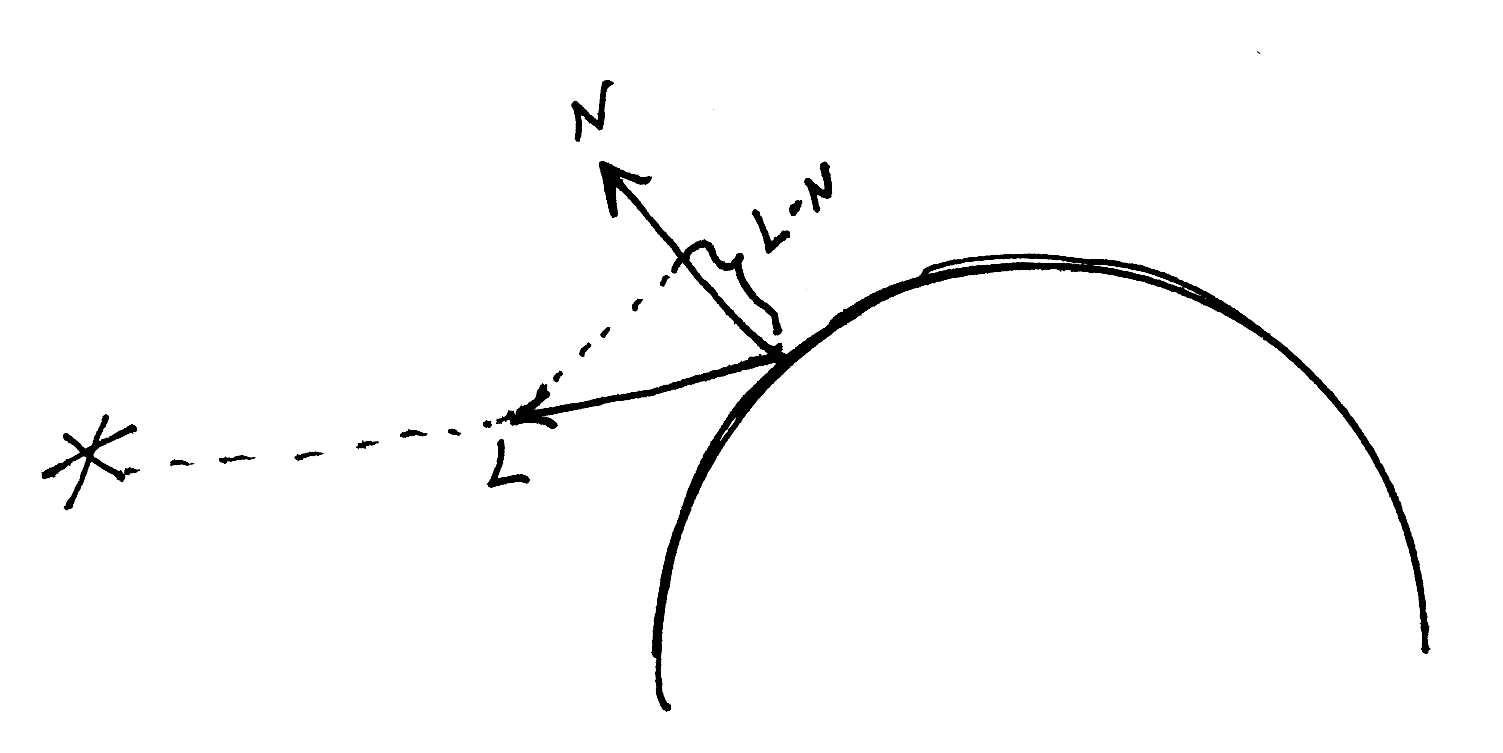
\includegraphics[width=2.5in]{images/diffuse.jpg}
\caption{Diffuse illumination is the dot product of two normalized vectors}
\end{figure}



\section{Specular illumination}
Specular illumination models the shininess of objects and is responsible for the bright spot on a
shiny apple or the glint off the chrome bumper of a car. It is largest when the light bouncing
off of the surface (assuming it was mirrored) would bounce directly into the camera and it falls
off rapidly as the camera moves away from that point of maximum specular intensity. The rate at
which it falls of is called the hardness. Lets now look at one way to model specular illumination.

Let ${\vect q}$ be a point on an object with normal ${\vect N}$ and let $\vect L$ be the unit vector that points
toward a light at position $\vect j$ and let $\vect E$ be the unit vector that points from ${\vect q}$ to the camera.
Let $P$ be the plane passing through ${\vect q}$ and with normal ${\vect N}$.

\begin{figure}[h]
\centering
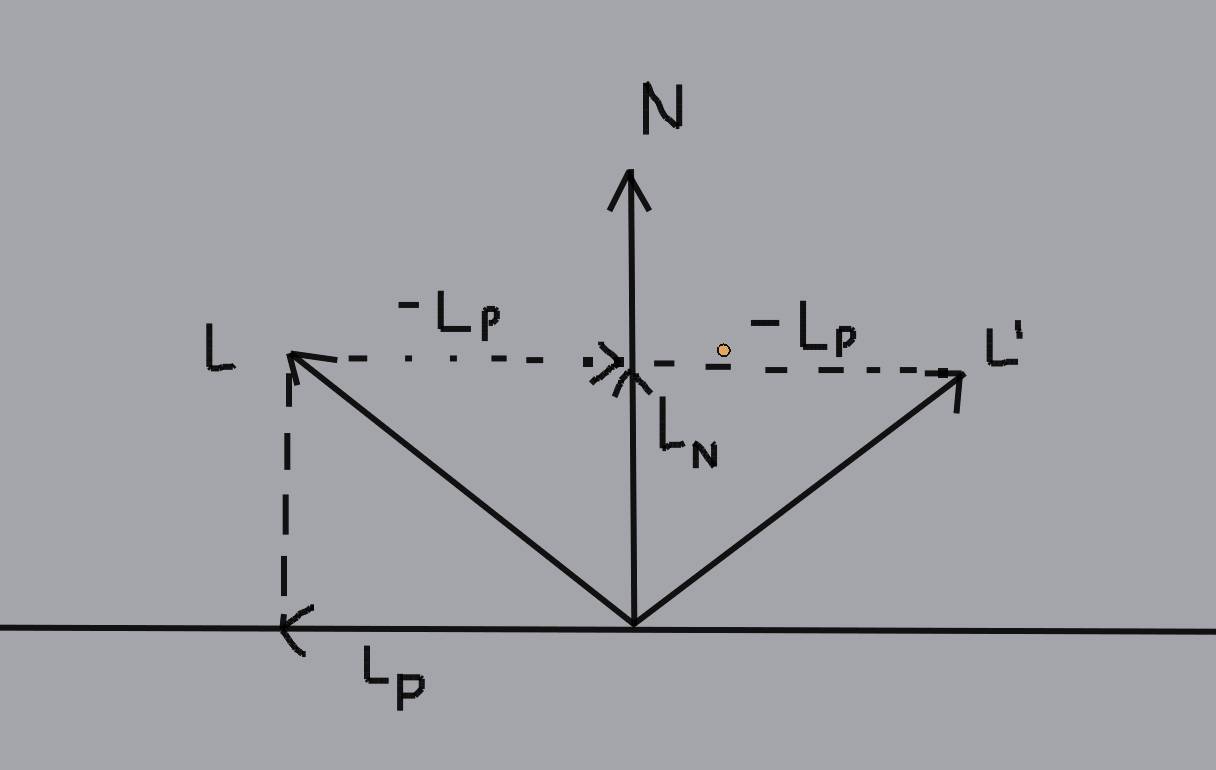
\includegraphics[width=2.5in]{images/reflection3.png}
\caption{Calculating the reflection of $\vect{L}$ relative to the normal $\vect{N}$ }
\end{figure}

The Phong model of specular illumination is computed by taking the cosine $c$ of the angle between ${\vect E}$ and
the reflection ${\vect L}'$ of ${\vect L}$ in $P$.
To compute $L'$ we first project $L$ onto ${\vect N}$ to get ${\vect L}_N$ and
also into a vector $L_P$ lying in $P$:
\begin{eqnarray*}
c &=& {\vect L} \cdot {\vect N}\\
{\vect L}_N &=& c {\vect N} \\
{\vect L}_P &=&  {\vect L} - {\vect L}_N \\
{\vect L}' &=& {\vect L} - 2 {\vect L}_P \;=\;  {\vect L} - 2 \left (  {\vect L} - {\vect L}_N     \right ) \\
&=&  2{\vect L}_N -{\vect L} \;=\;2 ({\vect L} \cdot {\vect N}) {\vect N} - {\vect L}
\end{eqnarray*}
The specular reflection, $s$, is then computed by calcuting $cos(\alpha)^n$ where $\alpha$
is the angle between $L'$ and $E$ and $h$ is the ``hardness'' of the material:
\[
s = ({\vect L'} \cdot {\vect E})^h
\]
The value $h$ is typically a small non-negative integer, e.g. between 0 and 511. Again, we assume that the light and the camera both appear above the plane $P$, that is ${\vect L}\cdot{\vect N}>0$ and ${\vect E}\cdot{\vect N}>0$; or both appear below the plane, making both dot products negative.   Otherwise, the specular illumination is zero.



The Blinn-Phong model is another way to calculate the specular reflection.
In this approach we find the vector $\vect W$ halfway between $\vect L$ and $\vect E$
and then use the angle $\beta$ between $\vect W$ and the normal $\vect N$ rather than $\alpha$. This gives
as value $s'$ which is another type of specular illumination:
\begin{eqnarray*}
{\vect W} &=& \frac{{\vect L}+{\vect E}}{\vert {\vect L} +{\vect E}\vert} \\
s' &=& ({\vect W} \cdot {\vect N})^h
\end{eqnarray*}

\begin{figure}[h]
\centering
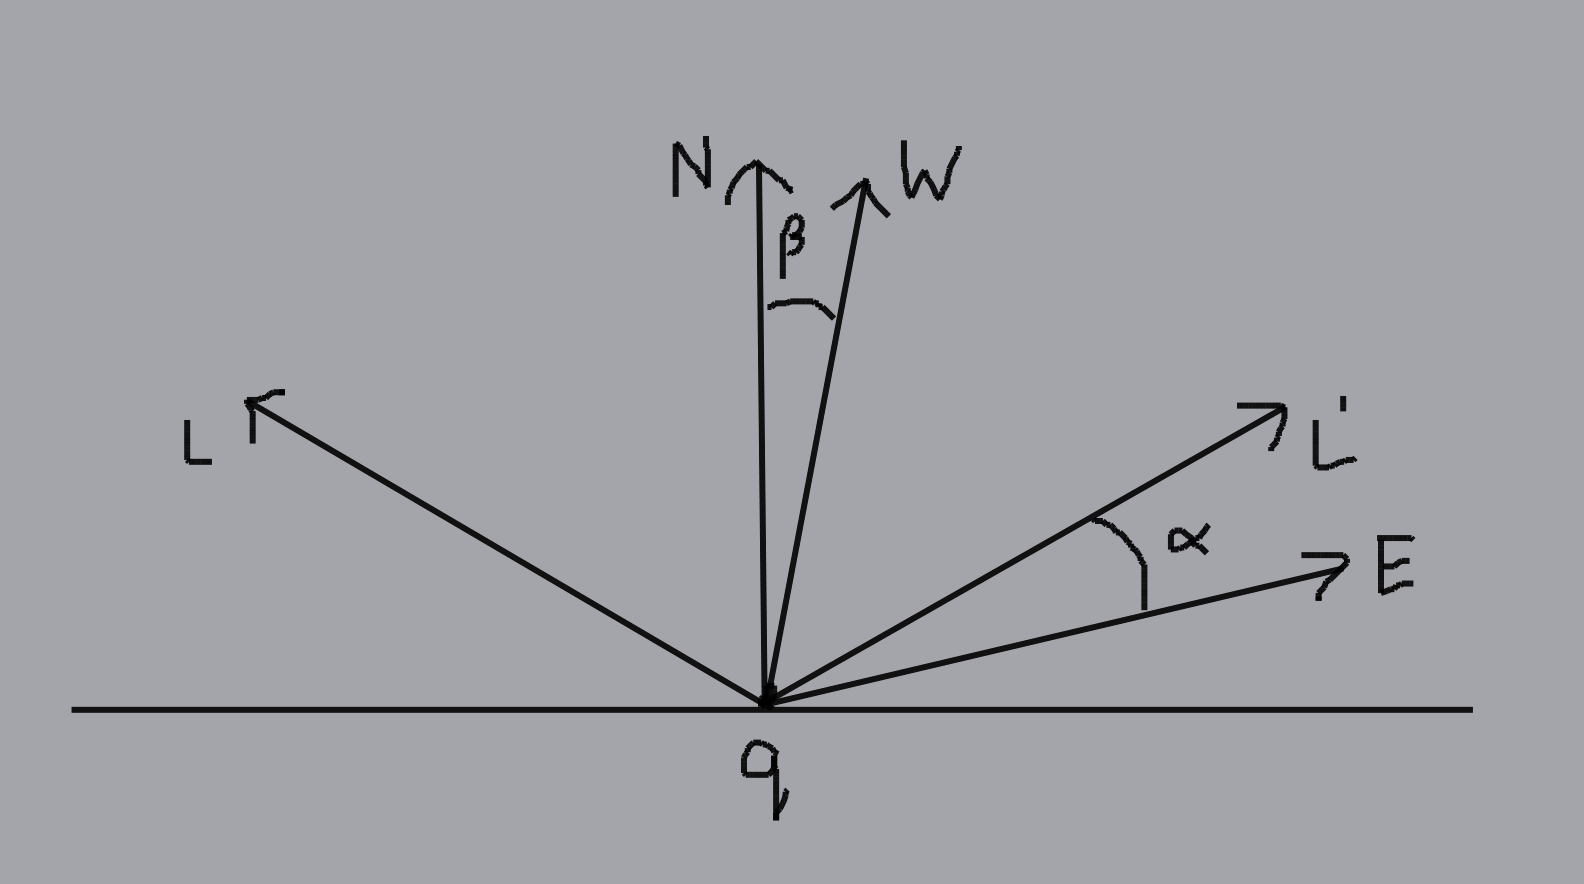
\includegraphics[width=2.5in]{images/specular1.png}
\caption{Specular illumination}
\end{figure}


\section{Lights}
The lights in this version of the ray tracer are specified by giving
their positions and intensities.
They also have methods to compute the diffuse and specular lighting intensities.
You might want to put these methods in the Material class instead...

The diffuse intensity depends on the normal to the object and the vector from the
intersection point to the light.
The specular intensity also needs to vector from the intersection point to the camera
and the hardness coefficient of the material.


\begin{figure}
\begin{verbatim}
\end{verbatim}

\caption{the Light Class \label{fig:LightClass}}
\end{figure}

\section{Color!}
In this Chapter we have considered a monochrome world with all colors being shades of gray from black (0.0) to white (1.0).  It is a relatively simple extension to represent colors as triples $(r,g,b)$ specifying the proportions of red, green, and blue in the color.   We leave it as an exercise to extend your code to handle colors as 3-tuples.



\chapter{Transforms \label{chap:transforms}}

One of the most useful tools in computer graphics is the notion of a transform
and the observation that one can easily find the intersection of ray with the transform
of an object, by intersecting the original object with the inverse transform of the ray,
and then applying the transform to the resulting point. In this section we show how to
represent a wide class of transforms as 4x4 matrices. In the next section, we'll show how
to compute the intersection of a ray with a transform of an object, and to compute the
normal at that point as well.

\section{Fundamental Transforms}
We will look at three classes of transforms: translations, rotations, and scalings,
and we will show how to represent all of these transforms as 4x4 matrices. Composing these
transforms can be done by multiplying their corresponding matrices and this gives us
a compact way of representing arbitrary combinations of translations, rotations, and scales.
The class of transforms that can be represented by 4x4 matrices are called the affine transforms
and they are heavily used in Computer Graphics.


\subsection{Translation}
For any point $p$ in 3D space, the translation $T_p$ is a function that maps a point $q$ to $p+q$:
\[
T_p(q) = p+q
\]
or in terms of vectors if $p = (a,b,c)$ then
\[
T_p(x,y,z) = (x+a, y+b, z+c)
\]
We represent $T_p$ by a 4x4 matrix:
\[
T_p =
\left (
\begin{array}{cccc}
1 & 0 & 0 & a \\
0 & 1 & 0 & b \\
0 & 0 & 1 & c \\
0 & 0 & 0 & 1
\end{array}
\right )
\]
To apply this matrix to a point $(x,y,z)$ we embed it in 4d space by adding a 1 in the fourth coordinate
and then apply the 4x4 transformation matrix to this 4-tuple as usual:
\[
T_p(x,y,z) =
\left (
\begin{array}{cccc}
1 & 0 & 0 & a \\
0 & 1 & 0 & b \\
0 & 0 & 1 & c \\
0 & 0 & 0 & 1
\end{array}
\right )
\left (
\begin{array}{c}
x \\
y \\
z \\
1 \\
\end{array}
\right )
=
\left (
\begin{array}{c}
x+a \\
y+b \\
z+c \\
1 \\
\end{array}
\right )
\]

To apply this matrix to a direction $(x,y,z)$ such as the direction $\vect{d}$ in a ray,
we embed it in 4d space by adding a 0 in the fourth coordinate
and then apply the 4x4 transformation matrix to this 4-tuple as usual:
\[
T_p(x,y,z) =
\left (
\begin{array}{cccc}
1 & 0 & 0 & a \\
0 & 1 & 0 & b \\
0 & 0 & 1 & c \\
0 & 0 & 0 & 1
\end{array}
\right )
\left (
\begin{array}{c}
x \\
y \\
z \\
0 \\
\end{array}
\right )
=
\left (
\begin{array}{c}
x \\
y \\
z \\
0 \\
\end{array}
\right )
\]
and we see that translating a direction in space does not change its value,
which is as we would expect.


\subsection{Scaling}
For any triple $p=(a,b,c)$, the scaling matrix $S_p$ is the following function
\[
S_p(x,y,z) = (a*x, b*y, c*z)
\]
We represent $S_p$ by a 4x4 matrix:
\[
S_p =
\left (
\begin{array}{cccc}
a & 0 & 0 & 0 \\
0 & b & 0 & 0 \\
0 & 0 & c & 0 \\
0 & 0 & 0 & 1
\end{array}
\right )
\]

\subsection{Rotation}
For any angle $a$, let $s = \sin(a)$ and $c=\cos(a)$. Then the
rotation transformation $R_{z,a}$ that rotates the point $q$ around the z-axis by the angle $a$ is given by
\[
R^z_a(x,y,z) = (c*x - s*y, s*x + c*y, z)
\]
which is represented by the following 4x4 matrix:
\[
R^z_a =
\left (
\begin{array}{cccc}
c & -s & 0 & 0 \\
s & c & 0 & 0 \\
0 & 0 & 1 & 0 \\
0 & 0 & 0 & 1
\end{array}
\right )
\]
Similary we can rotate around the y and x axes:
\[
R^y_a =
\left (
\begin{array}{cccc}
 c & 0 & s & 0 \\
 0 & 1 & 0 & 0 \\
-s & 0 & c & 0 \\
 0 & 0 & 0 & 1
\end{array}
\right )
\]
and
\[
R^x_a =
\left (
\begin{array}{cccc}
1 & 0 & 0 & 0 \\
0 & c & -s & 0 \\
0 & s & c & 0 \\
0 & 0 & 0 & 1
\end{array}
\right )
\]

\subsection{Compound Transformations}
A general 4x4 matrix $T$ represents a transform on both points $p=(x,y,z,1)$ in 3D space and
directions $p=(x,y,z,0)$ as follows.
First we apply $T$ to the point $p=(x,y,z,w)$ where $w$ is 1 for a point and 0 for a direction.
This gives us some vector $q=(a,b,c,d)$. If $d$ is non-zero then
\[
T(x,y,z) = (a/d, b/d, c/d, 1)
\]
otherwise $T(p)$ is a direction which we can think of as the ``point at infinity in the direction $(a,b,c,0)$''.

This space consisting of both regular points $p=(x,y,z,1)$ and points at infinity $p'=(x,y,z,0)$ is called
Projective 3 space. It can also be represented as the equivalence classes of points in 4D space where two
points are equivalent if one is a non-zero multiple of another.
\[
(x,y,z,w) \equiv (\lambda x, \lambda y, \lambda z, \lambda w)
\]
for all real numbers $\lambda \ne 0$. The representation of a 3D point or direction as a 4-tuple of numbers
is called homogeneous coordinates.

For example, lets consider the operation that rotates a point $p$ through the vector parallel to the z-axis that passes through the point $q$.
We can represent this as a composition of three operators. First translate by $-q$. This moves $q$ to the origin. Then rotate about the
$z-axis$, then translate by $q$ which moves the origin back to $q$. Thus, this operation is
\[
M^z_{q,a} = T_q R^z_a T_{-q}
\]
and if $q=(u,v,w)$ and $s = \sin(a)$ and $c=\cos(a)$, then we have
\begin{eqnarray*}
M^z_{q,a} &=&
\left (
\begin{array}{cccc}
1 & 0 & 0 & u \\
0 & 1 & 0 & v \\
0 & 0 & 1 & w \\
0 & 0 & 0 & 1
\end{array}
\right )
\left (
\begin{array}{cccc}
c & -s & 0 & 0 \\
s & c & 0 & 0 \\
0 & 0 & 1 & 0 \\
0 & 0 & 0 & 1
\end{array}
\right )
\left (
\begin{array}{cccc}
1 & 0 & 0 & -u \\
0 & 1 & 0 & -v \\
0 & 0 & 1 & -w \\
0 & 0 & 0 & 1
\end{array}
\right ) \\
&=&
\left (
\begin{array}{cccc}
c & -s & 0 & (1-c)u + sv \\
s & c & 0 & -su + (1-c)v \\
0 & 0 & 1 & 0 \\
0 & 0 & 0 & 1
\end{array}
\right )
\end{eqnarray*}
and this gives a matrix representation for a fairly complex compound operation.

\subsection{The general rotation around a vector v}
Let $\vect{v} = (v_x, v_y, v_z)$ be a non-zero vector and let $a$ be an angle. We want to find a matrix
that rotates points around an axis specified by the vector $v$. For example, when $v=(0,0,1)$ this should
just be the $R^z_a$ matrix that rotates around the z-axis.

There is a very clever way of constructing this matrix which we describe below.
Lets think of $v$ as a column vector:
\[
\vect{v} =
\left (
\begin{array}{c}
v_x\\
v_y\\
v_z
\end{array}
\right ) \\
\]
and lets normalize $\vect{v}$ so that it has length 1. That is $\vect{v}^T* \vect{v} = v_x^2+v_y^2+v_z^2 = 1$.
Next let $v^\flat$ be the matrix such that for any vector $\vect{w}$,
we have $v^\flat \cdot w = v \times w$, that is
\[
\vect{v}^\flat =
\left (
\begin{array}{ccc}
0& -v_z & v_y \\
v_z& 0 & -v_x \\
-v_y & v_x & 0 \\
\end{array}
\right ) \\
\]
Next, let $R = v*v^T$ be the dense 3x3 matrix obtained by multiplying $\vect{v}$ with itself
\[
R = v*v^T =
\left (
\begin{array}{c}v_x\\v_y \\ v_z \end{array}\right ) * (v_x v_y v_z) =
\left (
\begin{array}{ccc}
v_x^2 & v_xv_y & v_xv_z \\
v_yv_x & v_y^2 & v_yv_z \\
v_zv_x & v_zv_y & v_z^2
\end{array}
\right ) \\
\]
and let $I$ be the identity matrix as usual (i.e. the matrix with 1's down the diagonal and 0's elsewhere:
\[
I =
\left (
\begin{array}{ccc}
1 & 0 & 0 \\
0 & 1 & 0 \\
0 & 0 & 1
\end{array}
\right )
\]
Finally, let $c=\cos(a)$ and $s=\sin(a)$ and define $M$ to be the following matrix:
\begin{eqnarray*}
M &=& v*v^T + c(I-v*v^T) + s*v^\flat \\
\end{eqnarray*}
and so $M= $
\begin{eqnarray*}
&=& v*v^T + c(I-v*v^T) + s*v^\flat \\
&=&
\left (
\begin{array}{ccc}
v_x^2 & v_xv_y & v_xv_z \\
v_yv_x & v_y^2 & v_yv_z \\
v_zv_x & v_zv_y & v_z^2
\end{array}
\right )
+
\left (
\begin{array}{ccc}
c(1-v_x^2) & -cv_xv_y & -cv_xv_z \\
-cv_yv_x & c(1-v_y^2) & -cv_yv_z \\
-cv_zv_x & -cv_zv_y & c(1-v_z^2)
\end{array}
\right )
\\
&&
+
\left (
\begin{array}{ccc}
0& -sv_z & sv_y \\
sv_z& 0 & -sv_x \\
-sv_y & sv_x & 0 \\
\end{array}
\right ) \\
&=&
\left (
\begin{array}{ccc}
c+(1-c)v_x^2 & (1-c)v_xv_y - sv_z & (1-c)v_xv_z + s v_y \\
(1-c)v_yv_x+sv_z & c+(1-c)v_y^2 & (1-c)v_yv_z - sv_x \\
(1-c)v_zv_x  -sv_y& (1-c)v_zv_y +sv_x & c + (1-c)v_z^2
\end{array}
\right )
\end{eqnarray*}
and this gives a relatively simple matrix representation for a general rotation about a
general non-zero vector $v$.

\subsection{Proof of the general rotation formula}
Now let $p$ be any point, and let $w$ be the projection of $p$ into the plane perpendicular to $v$.
Then $p=v+w$ and $v^T*w=0$. Finally, let $u = v\times w$.
We will see that
\[
M(v+w) = v + cw + su
\]
which shows that $M$ rotates $p$ by an angle $a$ around $v$.

Proof:
First observe that $M(v)=v$ using $v*v^T*v = v*1 = v$ and $v^\flat*v = v\times v = 0$.
Indeed,
\begin{eqnarray*}
M(v) &=& (v*v^T + c(I-v*v^T) + sv^\flat)*v \\
 &=& (v*v^T)*v + c(I-v*v^T)*v + sv^\flat*v \\
 &=& v*(v^T*v) + cI*v -cv*v^T*v + sv^\flat*v \\
 &=& v*(v\cdot v) + (cv -cv*(v\cdot v)) + s(v \times v) \\
 &=& v + (cv-cv) + 0 \\
 &=& v
\end{eqnarray*}
Next observe that $M(w) = cw + su$ using $v^T*w=0$ and $v^\flat*w = v\times w = u$.
Indeed,
\begin{eqnarray*}
M(w) &=& (v*v^T + c(I-v*v^T) + sv^\flat)*w \\
 &=& v*v^T*w + cw-cv*v^T*w + sv^\flat*w \\
 &=& v*(v\cdot w) + cw-cv*(v\cdot w) + s(v \times w) \\
 &=& v*(0) + cw-cv*(0) + su \\
 &=&  cw + su \\
\end{eqnarray*}
as we set out to show.

\section{Applying a transform to a ray}
The use of 4x4 matrices allows us to represent translations, rotations, and scaling operations
as matrices provided we represent points in 3D space as 4-tuples where the last coordinate is 1.
This representation is called homogeneous coordinates. It has another advantage and that is that
by setting the last coordinate to 0, we can represent directions, and these are then handled correctly
by the usual matrix operations, that is, rotations and scaling operations modify the direction, but
translations have no effect. We can then apply a transform to a ray by simply representing the point $p$
and the direction $d$ of the ray in homogeneous coordinates and then applying the transform directly to
$p$ and $d$ respectively.

So if $\vect R = \vect{p}+t\vect{d}$ is a ray with $\vect{p} = (x,y,z,1)$ and $\vect{d} = (a,b,c,0)$, and $T$ is an affine transform, then
$T(\vect R(t)) = T(\vect{p})+t\;T(\vect{d})$.
% Equivalently, we can calculate $T(\vect d)$ as $T(\vect p+\vect d)-T(\vect p)$ since $d$ is the vector from $p$ to $p+d$.

\section{Intersecting a ray with a transformed object}
Given an object $X$ and a ray $R$ with origin $p$ and direction $d$, we want to find the number $t$ and the vector $n$ such that $R.p + t*R.d = T(q)$ is the closest intersection of $R$ with a point $T(q)$ of $T(X)$, and $N'$ is the normal at $T(q)$.


If $T$ is a transform, then $T(X)$ is the set of all points $\{T(x): x\in X\}$.
For example,
if $X$ is a sphere of radius 1 centered at the origin, then
\begin{itemize}
\item for any rotation $R$,  $R(X) = X$,
\item if $T=T_p$ is a translation, then $T_p(X)$ is the sphere of radius 1 centered at $p$,
\item if $S_{(a,b,c)}$ is a scaling operator, then $S_p(X)$ is an ellipsoid whose
x,y, and z axes have lengths $a,b,c$ respectively.
\end{itemize}

To compute the intersection of a ray $R$ with $T(X)$ we can apply a two step process:
\begin{itemize}
\item first compute the inverse $S$ of the transform $T$, i.e. the transform $S$ such that $S(T(x))=T(S(x))=x$ for all x,
\item then compute the intersection point $q$ of the inverse transformed ray $R'=S(R)$ with the untransformed object $X$
and calculate the normal vector $\vect N$ of $X$ at $q$.
\item then apply $T$ to $q$ to get the intersection $T(q)$ of $R$ with $T(X)$
\item finally calculate the normal $N'$ of $T(X)$ at $T(q)$
\end{itemize}

\subsubsection{Calculation of the normal of a transformed object}
You might think that we can calculate the normal $N'$ at $T(q)$ just by applying $T$ to $N$, but that doesn't work. In fact, you need to calculate it by applying the transpose of the inverse of T to $N$, that is $N' = (T^{-1})^t(N)$.

To see why observe that the transform $T$ does map tangent vectors on $X$ to tangent vectors on $T(X)$ because it maps pairs of nearby points on $X$ to pairs of nearby points on $T(X)$, hence it maps secants to secants and by passing to the limit, it maps tangents to tangents (assuming that the surface is "smooth" enough).

So $u$ is a vector which is tangent to the surface of $X$ at $q$ if and only if $ N \cdot u = 0$.  Applying $T$ to both sides we see that for every tangent vector $v$ at $q$ we get the following (where we assuming $N$ and $v$ are column vectors and $x^t$ is the transpose of $x$)
\[
0 =  N \cdot v = N^t * v = N^t * (S*T)*v = (N^t*S) * T*v = (S^t*N^t)^t * T*v = S^t(N) \cdot T(v)
\]
so $S^t(N)$ is perpendicular to all tangent vectors of $T(X)$ at $T(q)$ and hence it must be the normal.
Thus, $N' = S^t(N) = (T^{-1})^t(N)$.

\subsubsection{Calculation of the distance parameter $t'$}
Once we have calculated the intersection point $T(q)$ we can find the distance using of the ray origin $R.p$ to $T(q)$ easily. We can also calculate the "distance" from the corresponding distance for the inverse transformed ray.
That is we will have found a $t$ such that $S(R.p) + t*S(R.d) = q$.  Applying $T$ to both sides we get
\[
R.p + t*R.d = T(q)
\]
So if we don't normalize the ray directions $S(R.d)$ to have length 1, then the "distance" at which the ray $S(R)$ hits the object $X$ is the same as the "distance" at which the ray $R$ hits $T(X)$.  If we do normalize ray lengths, and let $d'$ be the length of $S(R.d)$, then we would have
\[
S(R.p) + t'*S(R.d)/d' = q
\]
So applying $T$ to both sides we get
\[
R.p + (t'/d')*R.d = T(q)
\]
So we need to divide $t'$ by $d'$ to get the "distance" $t$ along the ray $R$ at which it intersects $T(X)$.



\section{Exercises}
Let $h = \frac{\sqrt{2}}{2}$, so $h = \sin(\pi/4)$.
\begin{enumerate}
\item Write out the transformation matrix $R_z$ which rotates the world around the z axis by 45 degrees.
\item Write out the transformation matrix $R'_z$ which rotates the world around the z axis by -45 degrees.
\item Write out the transformation matrix $R_y$ which rotates the world around the $y$ axis by 45 degrees.
\item Write out the transformation matrix $T$ which translates the origin to the point $(1, 2, 3)$
\item Write out the transformation matrix $S$ which scales $(x,y,z)$ to $(2x, 2y, 3z)$
\item Compute the matrix product $R_z R'_z$.
\item Compute the matrix products $R_y R_z$ and also $R_z R_y$? Are they equal? If not, how are they different?
\item Compute the matrix products $R_z S$ and $S R_z$? Are they equal?
\item Apply the matrix $S T$ to the vector $(-2,3,1)$
\end{enumerate}



\chapter{More Objects}

\section{Adding planes to the ray tracer}

\subsection{Constraint for a point to be in a plane}
A plane $P$ can be specified by a point ${\vect q}$ and a normal ${\vect m}$ to that plane.
A point ${\vect v}$ is in the plane if the vector ${\vect v} - {\vect q}$ is perpendicular to ${\vect m}$.
That is if
\[
({\vect v} - {\vect q})\cdot {\vect m} = 0
\]

\subsection{Intersecting a ray with a plane in vector notation}
To determine the intersection of a ray $r_{{\vect p},{\vect d}}$
with a plane passing through ${\vect q}$ and with normal ${\vect m}$, we look for points ${\vect v}$ on the
plane which are also on the ray, and hence have the form: ${\vect p} + t {\vect d}$
\begin{eqnarray*}
0 &=& ({\vect v} - {\vect q}) \cdot {\vect m}\\
 &=& (t {\vect d} + {\vect p} - {\vect q}) \cdot {\vect m}\\
 &=& t {\vect d} \cdot {\vect m} \;+\; ({\vect p} - {\vect q}) \cdot {\vect m} \\
\end{eqnarray*}
So, solving for $t$ we get
\[
t = \frac {({\vect q} - {\vect p})\cdot m} {{\vect d} \cdot {\vect m}}
\]
provided ${\vect d} \cdot {\vect m} \ne 0$.
If $t>0$, then the ray interesects the plane.


\begin{figure}
\begin{verbatim}

\end{verbatim}
\caption{Plane Class \label{fig:PlaneClass}}
\end{figure}



\section{Adding cylinders to the ray tracer}
In this section, we specify a cylinder by two vectors and two positive numbers.
\begin{itemize}
\item a point ${\vect q}$ at the center of the base of the cylinder
\item a vector ${\vect m}$ that defines the central axis of the cylinder
\item the radius $r$ of the cylinder, and
\item the height $h$ of the cylinder
\end{itemize}
We first find a formula for testing whether a point $v$ is on the cylinder.
The idea is to project the point $v$ onto a the plane $P$ through $q$ with normal $m$.
This gives a point $v_2$ on the plane $P$. If the distance between $v_2$ and $q$ is $r$
then the point is on the infinite tube containing the cylinder in question:
\begin{eqnarray*}
{\vect v}_1 &=& {\vect v} - {\vect q} \\
{\vect v}_2 &=& {\vect v}_1 - ({\vect v}_1 \cdot {\vect m}) {\vect m} \\
\vert {\vect v}_2 \vert^2 &=& r^2
\end{eqnarray*}
To see if
it is on the cylinder we must do two more tests using ${\vect v}_1$:
\begin{eqnarray*}
{\vect v}_1 \cdot {\vect m} & \ge & 0 \\
{\vect v}_1 \cdot {\vect m} & \le & h
\end{eqnarray*}
\subsection{Intersecting the cylinder with a ray}
We now plug in ${\vect v} = t {\vect d} + {\vect p}$ into the cylinder test above and
solve for $t$. This will give a quadratic equation that we can solve for two roots $t_1$ and $t_2$.
Then we find the smallest of these two roots whose corresponding point $v$ also satisfies the
two dot product constraints.
\begin{eqnarray*}
{\vect v} &=& t {\vect d} + {\vect p} \\
{\vect w} &=& {\vect p} - {\vect q} \\
{\vect v}_1 &=& t {\vect d} + {\vect w} \\
{\vect v}_1 \cdot {\vect m}  &=& t ({\vect d}\cdot {\vect m}) + {\vect w}\cdot {\vect m} \\
{\vect v}_2 &=& {\vect v}_1 - ({\vect v}_1 \cdot {\vect m}){\vect m} \\
  &=& t {\vect d} + {\vect w}  - (t {\vect d} \cdot {\vect m} + {\vect w}\cdot {\vect m}){\vect m} \\
  &=& t ({\vect d} - ({\vect d} \cdot {\vect m}) {\vect m}) + {\vect w}  - ({\vect w}\cdot {\vect m}){\vect m} \\
 &=& t {\vect \alpha} + {\vect \beta}  \\
\end{eqnarray*}
where
\begin{eqnarray*}
{\vect \alpha}  &=& {\vect d} - ({\vect d} \cdot {\vect m}) {\vect m} \\
{\vect \beta} &=&  {\vect w}  - ({\vect w}\cdot {\vect m}){\vect m}  \\
\end{eqnarray*}
so the point ${\vect v}$ is on the cylinder if and only if
\begin{eqnarray*}
r^2 &=& \vert {\vect v}_2 \vert^2 \\
&=& t^2 \vert {\vect \alpha} \vert^2 + t 2 {\vect \alpha} \cdot {\vect \beta} + \vert {\vect \beta} \vert^2
\end{eqnarray*}
which is a quadratic in the variable $t$
\[
A^2 + Bt + C = 0
\]
This quadratic has a solution iff the discriminant $D = B^2 -4AC$ is non-negative
where
\begin{eqnarray*}
A &=& \vert {\vect \alpha}\vert^2 \\
B &=&  2 {\vect \alpha} \cdot {\vect \beta} \\
C &=& \vert {\vect \beta} \vert^2 - r^2
\end{eqnarray*}
The quadratic formula gives two solutions $t_1$ and $t_2$ which corresponds to
two points ${\vect u}_1 = t_1 {\vect d} + {\vect p}$ and ${\vect u}_2 = t_2 {\vect d} + {\vect p}$.
We look for the smallest $t_i$ which is positive and for which $({\vect u}_i - {\vect q}) \cdot {\vect m} \ge 0$ and
$({\vect u}_i  - {\vect q}) \cdot {\vect m} \le h$. If there are no such $t_i$ then the ray does not intersect the cylinder;
otherwise the selected $u_i$ is the intersection point.

\subsection{Finding the normal to a cylinder at a point}
To find the normal ${\vect n}$ at a point $v$ on a cylinder, we just project it into the plane
perpendicular to the central axis ${\vect m}$ of the cylinder.
\begin{eqnarray*}
{\vect v}1 &=& {\vect v} - {\vect q} \\
{\vect n} &=&  {\vect v}1 - ({\vect v}1 \cdot m) {\vect m}
\end{eqnarray*}


\begin{figure}
\begin{verbatim}

\end{verbatim}
\caption{Cylinder Class \label{fig:CylinderClass}}
\end{figure}







\chapter{Reflection and Refraction}
\section{Reflection}
To find the reflection of a ray ${\vect d}$ at a point ${\vect q}$ of a plane $P$
with normal ${\vect n}$. We first project ${\vect d}$ onto the normal to get
\[
{\vect d}_n = ({\vect d}\cdot{\vect n}) {\vect n}
\]
This vector represent how far beneath the plane the ray would go if it passed straight
through the plane. To get the reflection we add twice ${\vect d}_n$ to {\vect d} and get
the reflection direction:'\
\[
{\vect d'} = {\vect d} - 2 {\vect d}_n
\]
The reflecting ray starts at point ${\vect q}$ and goes in direction ${\vect d'}$.
\begin{figure}[h]
\centering
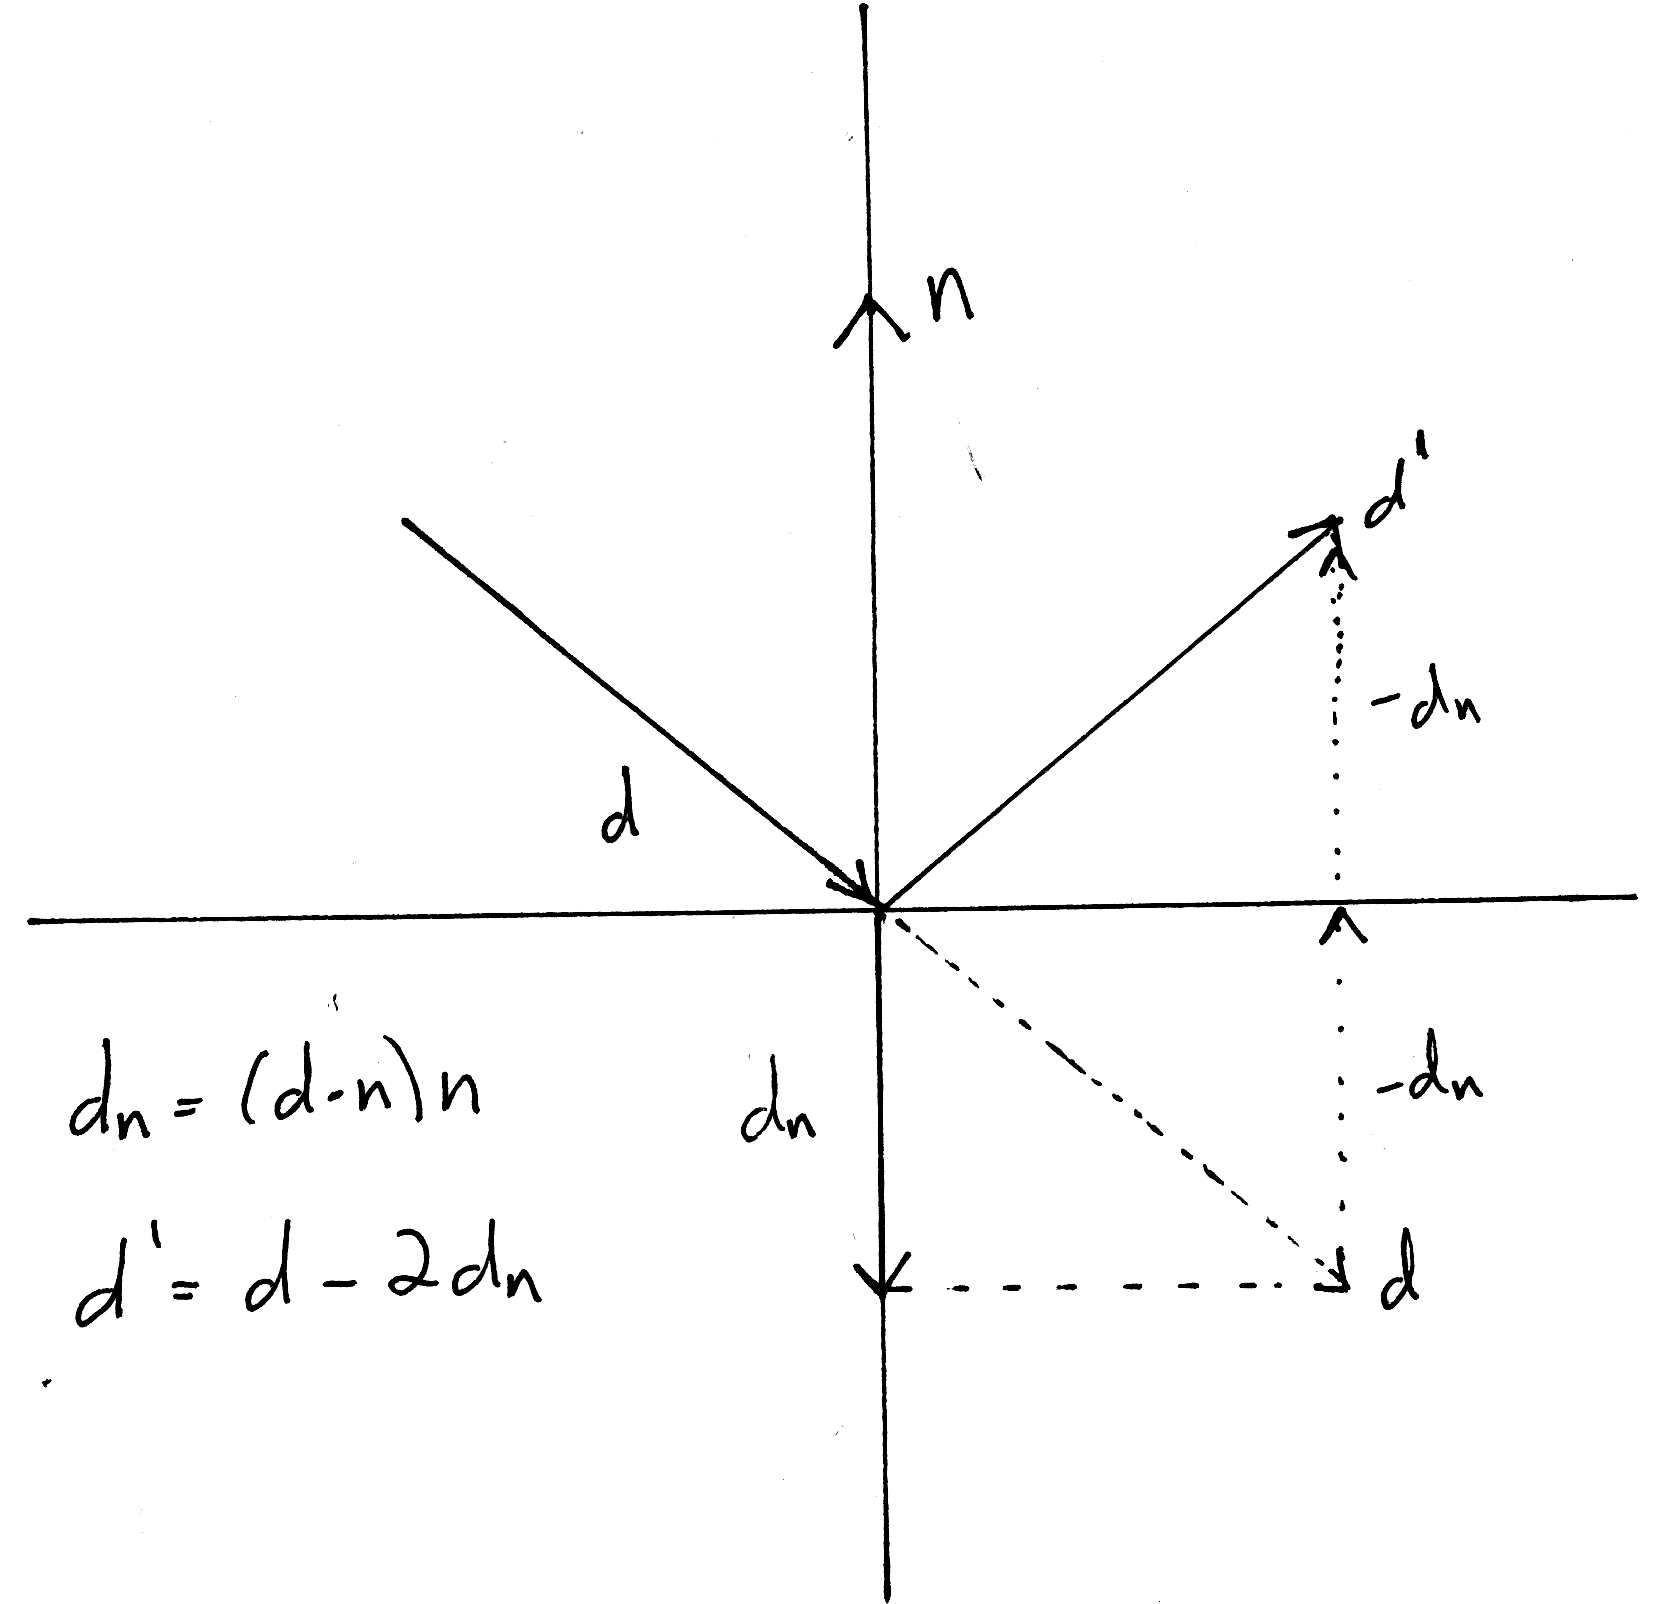
\includegraphics[width=2.5in]{images/reflection2.jpg}
\caption{Reflection of a Ray in a Surface}
\end{figure}
Note that this formula is different than the one we obtained in the previous section
when computing the specular reflection, because in that case we used a vector pointing
toward the light which was in the same direction as the normal. In this section
we are considering a vector pointing into the plane in the opposite direction of
the normal, if you let $\vect{e} = -\vect{d}$, and substitute into the formula
in this section, you'll get the same formula as in the previous section.



\section{Refraction}
Light travels at different speeds in different media. The index of refraction (IOR) of a material
is a number related to the speed of light in that material.
when light passes from one region to another with a different index of refraction (IOR)
the light ray is bent in a way that depends on the two IORs. Indeed, if we let $a_1$ be
the angle between the entering ray and the outward facing normal $\vect{N}$, and let $a_2$ be the
angle between the exiting ray and the inward facing normal, and if we let $n_1$ and $n_2$ be
the two indices of refraction, then Snell's Law (shown below) describes the relationship
between these quantities:
\[
n_1 \sin(a_1) = n_2 \sin(a_2)
\]

\begin{figure}[h]
\centering
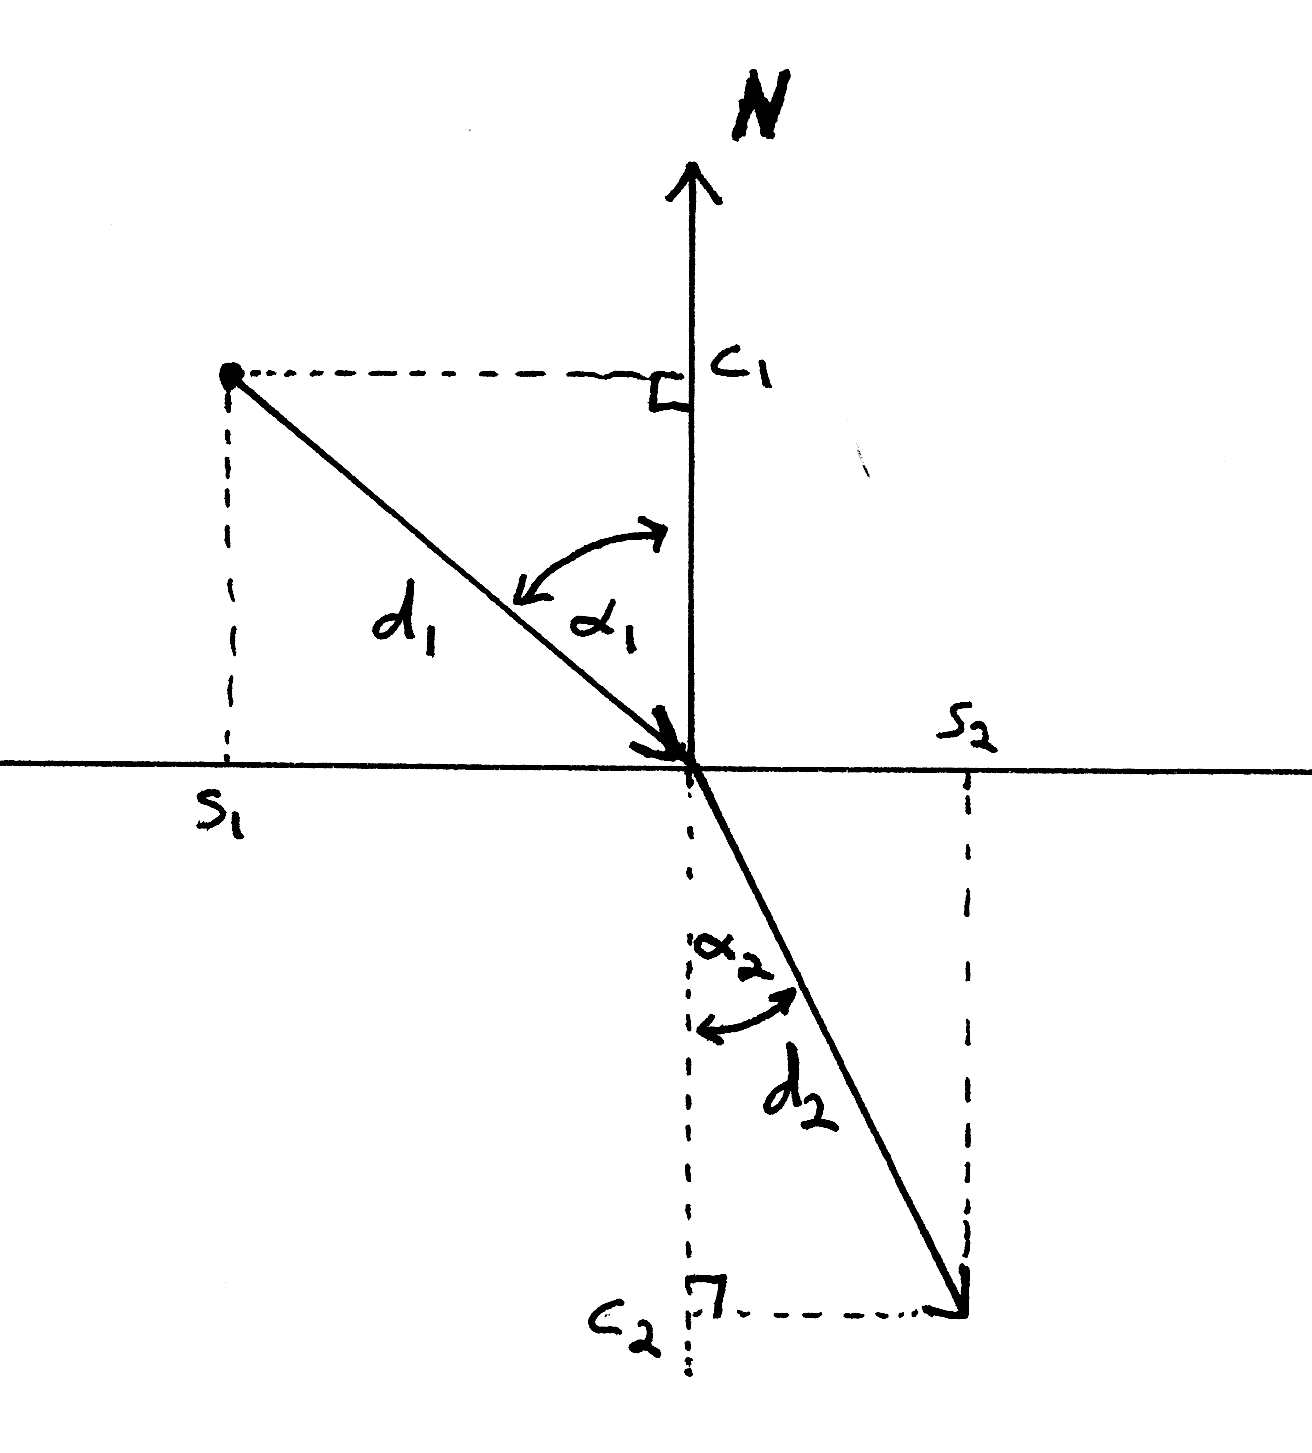
\includegraphics[width=2.5in]{images/refraction.jpg}
\caption{Refraction}
\end{figure}



Let ${\vect d}_1$ be the direction of the entering ray and ${\vect d}_2$ be the direction of the exiting ray.
If the IORs are equal, then ${\vect d}_1= {\vect d}_2$. Otherwise, we will usually know ${\vect d}_1$
and want to compute ${\vect d}_2$. The key to deriving this relation is by observing that
we can compute $c_1 = \cos(a_1)$ as a dot product between ${\vect d_1}$ and ${- \vect n}$.
This allows us to compute $s_1 = \sin(a_1)$ since $s_1^2 + c_1^2 = 1$
\begin{eqnarray*}
c_1 &=& {\vect d_1} \cdot {- \vect N} \\
s_1 &=& \sqrt{1 - c_1^2}
\end{eqnarray*}
Next, let $s_2 = \sin(a_2)$ and $c_2 = \cos(a_2)$ and $n = n_1/n_2$, then $s_2^2 + c_2^2 = 1$ and
from Snell's Law we know that $s_2 = n s_1$, so we can calculate $s_2$ and $c_2$ as
\begin{eqnarray*}
s_2 &=& n s_1 \\
c_2 &=& \sqrt{1 - s_2^2} \\
   &=& \sqrt{1 - n^2(1 - c_1^2)} \\
   &=& \sqrt{1 - n^2 + n^2 c_1^2} \\
\end{eqnarray*}



We can now express the refracted array in terms of two components. The component in the normal
direction is $- c_2 {\vect N}$ and the other part is the component in the plane $P$. To get this
we must first project ${\vect d}_1$ into $P$ to get a vector $\vect{f}_1$
and normalize it to get $\vect{f}_1/s_1$ of length one:
\begin{eqnarray*}
{\vect f}_1 &=& {\vect d}_1 - ({\vect d}_1 \cdot (- {\vect N}))(- {\vect N}) \\
&=& {\vect d}_1 - ({\vect d}_1 \cdot  {\vect N}) {\vect N} \\
&=& {\vect d}_1 + c_1 {\vect N} \\
\end{eqnarray*}
and so
\begin{eqnarray*}
{\vect d}_2 &=& c_2 (- {\vect N}) + s_2 {\vect f_1}/s_1 \\
 &=& - c_2{\vect N} + s_2/s_1 ({\vect d}_1 + c_1{\vect N}) \\
 &=& - c_2{\vect N} + n {\vect d}_1 + n c_1 {\vect N} \\
 &=&  n {\vect d}_1 +  (n c_1 - c_2) {\vect N} \\
\end{eqnarray*}
This gives us our final formula for the refraction direction ${\vect d}_d$ of a ray with direction ${\vect d}_1$
\[
{\vect d}_2  =  n {\vect d}_1 +  (n c_1 - c_2) {\vect N}
\]

\chapter{Textures}

Photorealism is greatly enhanced by adding textures to the geometric objects
and meshes in our raytracer. The approach described here is to associate
a texture coordinate with each intersection point of a ray and a surface.
The texture coordinate consists of a pair of floating point numbers which can
then be mapped to a color based on the particular texture associated with the
material.

The standard approach is to define a texture map on the plane which associates
an RGB color to any pair of floatin point numbers $(x,y)$. We can then get a texture
on an object by mapping each point ${\vect p}$ on the object to a point $(x,y)$ in
texture space, and using the texture color for that point.
% A more sophisticated
% approach would map each intersection point to a region of the texture space ...


\section{Textures for a cube}
The simplest way to create a texture map for a cube is to define the cube as
a group of transformed unit squares $([0,1],[0,1],0)$ in the $z=0$ plane.
The texture coordinate for a point $(x,y,0)$ is just $(x,y)$

\section{Texture mapping for the plane}
For the plane $z=0$ we can easily map an intersection point $(x,y,0)$ to the
natural texture coordinate $(x,y)$. For a general plane that passes through
a point ${\vect q}$ with normal ${\vect n}$ we can get the same effect by specifying two
orthogonal unit vectors in the plane (call them ${\vect r}$ for right and ${\vect u}$ for up
and then mapping a point ${\vect p}$ in the plane to its coordinates relative to the right and up
vectors:
\[
{\vect p} \mapsto (({\vect p}-{\vect q})\cdot {\vect r}, {(\vect p}-{\vect q})\cdot {\vect u})
\]
We can construct ${\vect r}$ by projecting some vector, say $(1,0,0)$ into the plane through $(0,0,0)$
with normal ${\vect n}$ to get ${\vect r}$. We can then get ${\vect u}$ using the cross product
\[
{\vect u} = {\vect n}\times{\vect r}
\]
as this will be orthogonal to ${\vect n}$ and hence in the plane, and will be orthogonal to ${\vect r}$
so the texture will be applied without any slant!  The one case where this approach may fail is when
$(1,0,0)$ is nearlly perpendicular to the plane, but in this case we can project $(0,1,0)$ instead as the
{\it right} vector.

\section{Texture mapping for the cylinder}
A cylinder is defined by the base plane (a point ${\vect q}$ and a normal ${\vect n}$) together with
a radius $R$ and a height $H$.

We can easily get a texture coordinate for an intersection point ${\vect p}$ on the cylinder by
projecting ${\vect p}$ into the base plane of the cylinder to get a point ${\vect p}'$.
\[
{\vect p}' =
{\vect p} -
(({\vect p} - {\vect q}) \cdot {\vect n})
{\vect n}
\]
Since the
projection is in the plane, it has a texture coordinate $(x,y)$ where
\begin{eqnarray*}
x &=& ({\vect p}-{\vect q})\cdot {\vect r} \\
y &=& ({\vect p}-{\vect q})\cdot {\vect u}
\end{eqnarray*}
where ${\vect r}$ and ${\vect u}$ are the {\tt right} and {\tt up} vectors
in the plane that define the texture of the plane as in the previous section.
We can use the {\tt atan2}
Java method to convert this into an angle $\alpha$ between $-\pi$ and $\pi$ radians.
\[
\alpha = {\tt Math.atan2}(y,x)
\]
To get the natural
texture coorindates for the cylinder, we can also compute the distance
\[
h = ({\vect p}- {\vect q})\cdot {\vect n}
\]
between the two points ${\vect p}$ and ${\vect p}'$, and then we get the texture coordinate
map
\[
{\vect p} \mapsto (h/H,1/2 + \alpha/(2\pi))
\]
which has the effect of unrolling the cylinder onto the plane and rescaling so it fits in the rectangle $[0,1]\times[0,1]$.

\section{Texture Coordinates for a sphere}
For simplicity, lets first consider a sphere centered at the origin.
The easiest way to get texture coordinates for the sphere is to circumscribe the sphere with a cylinder parallel to the y-axis
and then project the sphere onto the cylinder using rays perpendicular to the y-axis. For example,
let $S$ be a sphere with center ${\vect q}=(0,0,0)$ and radius $R$ and let ${\vect p}=(x,y,z)$ be a point on $S$.
Then $x^2 + y^2 + z^2 = R^2$ and the projection of this point onto the cylinder of radius $R$ perpendicular to the y axis
is
\[
(x/d,y/d,z)
\]
where $d = \sqrt{x^2+y^2}/R$ as then we have
\[
(x/d)^2 + (y/d)^2 = (x^2 + y^2)/d^2 = R^2
\]
We can then compute the texture coordinates for this point on the cylinder.

Another approach is to enclose the sphere in a box and project the sphere on the box using the normal
vectors of the sphere (actually this works with any geomatric shape that can be enclosed in a box).
A texture for the box then maps to a texture for the sphere.

\section{Texture transforms}
We have shown how to define an initial texture mapping for an object, but in practice one often
wants to transform the texture mapping. For example, shifting it, rotating it, scaling it, shearing it.
This can easily be implemented by defining a texture transform object which is a 2D affine transform
that is applied to the texture coordinates before the color is computed.

\bibliography{references}

\backmatter




\appendix

\chapter{Solutions to Exercises}
\section{Chapter \ref{chap:prelim}}

Consider the following three points
\begin{eqnarray*}
a &=& (1, 2, 2) \\
b &=& (7, -2, 4) \\
c &=& (0, 4, -2) \\
d &=& (1, 1, 1)
\end{eqnarray*}
Let $u$ be the vector from b to a, and let $v$ be the vector from b to c.
Let $P$ be the plane that passes through $d$ and is normal to $a$.
\begin{enumerate}
\item How long is the vector $u$?
\newline
\begin{eqnarray*}
u = a-b &=&= (1,2,2)- (7,-2,4) = (-6, 4, -2) \\
\vert u \vert &=& \sqrt{\vert u \cdot \vert} = \sqrt{36+16+4} = \sqrt{56}
\end{eqnarray*}

\item Is the angle between u and v less than 90 degrees, equal to 90 degrees, or greater than 90 degrees? How do you know?
\newline
Let $\theta$ be the angle between $\vect u$ and $\vect v$, and recall tha the dot product formula
expresses the dot product of two vectors in term of their lengths and the cosine of the angle between them:
\[
  \vect{u}\cdot \vect{v} = \vert \vect{u} \vert \;  \vert \vect{v} \vert \cos(\theta)
\]
If $\cos(\theta) > 0$, then $\theta$ must be less than 90 degrees and if $\cos(\theta) < 0$ then $\theta$ is greater than
90 degrees. So we compute:
\begin{eqnarray*}
u &=& (-6,4,-2) \\
v &=& c-b = (0,4,-2)- (7,-2,4) = (-7,6,-6) \\
u\cdot v &=& 42 + 24 + 12 = 78 > 0
\end{eqnarray*}
and see that the angle is less than 90 degrees.

\item Calculate the normalization of the vector $a$, i.e. the unit vector pointing in the same directions as $a$.
\newline
Since ${\vect{a}} = (1,2,2)$, $\vert \vect{a} \vert = \sqrt{1+4+4} = 3$ so the normalization $\tilde{\vect{a}}$ is
\[
\tilde{\vect{a}} = \frac{a}{3} = (\frac{1}{3},\frac{2}{3},\frac{2}{3})
\]
\item How far away is the point $b$ from the plane $P$?
\newline
To do this, we take the dot product of $w = \vect {b} - \vect {d}$ with $\tilde{\vect{a}}$
\[
w = (7,-2,4) - (1,1,1) = (6,-3,3)
\]
So
\[
\vect{w} \cdot \tilde{\vect{a}} = (6,-3,3) \cdot  (\frac{1}{3},\frac{2}{3},\frac{2}{3}) =
2 + (-2) + 2 = 2
\]
So $\vect{b}$ is 2 units above $P$.
\item Find the point $p$ which is the projection of $b$ onto the plane $P$.
\newline
We have already calculated that $\vect b$ is 2 units above $P$ where the notion of up
and down is specified by the normal $\tilde \vect a$.
Thus if we subtract t times the normal to $P$ from $b$ we will move it directly into the
plane, and this is the projection:
\[
\vect p = \vect b - ((\vect b - \vect d) \cdot \tilde \vect a) \tilde \vect a = (7,-2,4) - 2 (\frac{1}{3},\frac{2}{3},\frac{2}{3})
= (6\frac{1}{3}, -3\frac{1}{3},2\frac{2}{3})
\]

\item Use the cross product to find a vector $w$ which is perpendicular to $u$ and $v$.
\newline
\begin{eqnarray*}
u &=& (-6, 4, -2) \\
v &=& ( -7, 6, -6) \\
u\times v &=& (u_yv_z-u_zv_y, u_zv_x-u_xv_z, u_xv_y-u_zv_x) \\
&=& (-24--12, 14-36,-36--28) = (-12,-22,-8)
\end{eqnarray*}
and we can then check that $(4,2,-50)$ is perpendicular to $u$ and $v$:
\begin{eqnarray*}
(-6,4,-2) \cdot (-12,-22,-8) &=& 72 - 88 +16 = 0 \\
(-7,6,-6) \cdot (-12,-22,-8) &=& 84 -132 + 48 = 0
\end{eqnarray*}
\item Find the point $e$ that you get by rotating the point $c$ around the $x$ axis by 90 degrees.
\newline
Rotating $c = (0,4,-2)$ around the $x$ axis will keep the $x$ coordinate the same but will move the $y$ axis
onto the $z$ axis, and the $z$ axis onto the $-y$ axis, thus it should go to $(0, 2, 4)$.
\end{enumerate}

\section{Chapter \ref{chap:transforms}}

Let $h = \frac{\sqrt{2}}{2}$, so $h = \sin(\pi/4)$.
\begin{enumerate}
\item Write out the transformation matrix $R^z_{45}$ which rotates the world around the z axis by 45 degrees.
\[
R^z_{45} =
\left (
\begin{array}{cccc}
h & -h & 0 & 0 \\
h & h & 0 & 0 \\
0 & 0 & 1 & 0 \\
0 & 0 & 0 & 1
\end{array}
\right )
\]
\item Write out the transformation matrix $R^z_{-45}$ which rotates the world around the z axis by -45 degrees.
\[
R^z_{-45} =
\left (
\begin{array}{cccc}
h & h & 0 & 0 \\
-h & h & 0 & 0 \\
0 & 0 & 1 & 0 \\
0 & 0 & 0 & 1
\end{array}
\right )
\]
\item Write out the transformation matrix $R^y_{45}$ which rotates the world around the $y$ axis by 45 degrees.
\[
R^y_{45} =
\left (
\begin{array}{cccc}
 h & 0 & h & 0 \\
 0 & 1 & 0 & 0 \\
-h & 0 & h & 0 \\
 0 & 0 & 0 & 1
\end{array}
\right )
\]
\item Write out the transformation matrix $T$ which translates the origin to the point $(1, 2, 3)$
\[
T =
\left (
\begin{array}{cccc}
1 & 0 & 0 & 1 \\
0 & 1 & 0 & 2 \\
0 & 0 & 1 & 3 \\
0 & 0 & 0 & 1
\end{array}
\right )
\]
\item Write out the transformation matrix $S$ which scales $(x,y,z)$ to $(2x, 2y, 3z)$
\[
S =
\left (
\begin{array}{cccc}
2 & 0 & 0 & 0 \\
0 & 2 & 0 & 0 \\
0 & 0 & 3 & 0 \\
0 & 0 & 0 & 1
\end{array}
\right )
\]


\item Compute the matrix product $R^z_{45} R^z_{-45}$.
\begin{eqnarray*}
R^z_{45}  * R^z_{-45}  &=&
\left (
\begin{array}{cccc}
h & -h & 0 & 0 \\
h & h & 0 & 0 \\
0 & 0 & 1 & 0 \\
0 & 0 & 0 & 1
\end{array}
\right )
*
\left (
\begin{array}{cccc}
h & h & 0 & 0 \\
-h & h & 0 & 0 \\
0 & 0 & 1 & 0 \\
0 & 0 & 0 & 1
\end{array}
\right )
\\
&=&
\left (
\begin{array}{cccc}
h^2+h^2 & h^2-h^2 & 0 & 0 \\
h^2-h^2 & h^2+h^2 & 0 & 0 \\
0 & 0 & 1 & 0 \\
0 & 0 & 0 & 1
\end{array}
\right )
\\
&=&
\left (
\begin{array}{cccc}
1 & 0 & 0 & 0 \\
0 & 1 & 0 & 0 \\
0 & 0 & 1 & 0 \\
0 & 0 & 0 & 1
\end{array}
\right )
\end{eqnarray*}
since $h^2 = \frac{1}{2}$

\item Compute the matrix products $R^y_{45} R^z_{45}$ and also $R^z_{45} R^y_{45}$? Are they equal? If not, how are they different?
\begin{eqnarray*}
R^y_{45} * R^z_{45} &=&
\left (
\begin{array}{cccc}
 h & 0 & h & 0 \\
 0 & 1 & 0 & 0 \\
-h & 0 & h & 0 \\
 0 & 0 & 0 & 1
\end{array}
\right )
*
\left (
\begin{array}{cccc}
h & -h & 0 & 0 \\
h & h & 0 & 0 \\
0 & 0 & 1 & 0 \\
0 & 0 & 0 & 1
\end{array}
\right ) \\
&=&
\left (
\begin{array}{cccc}
h^2 & -h^2 & h & 0 \\
h & h & 0 & 0 \\
-h^2 & h^2 & h & 0 \\
0 & 0 & 0 & 1
\end{array}
\right )
\end{eqnarray*}
while
\begin{eqnarray*}
R^z_{45} * R^y_{45}
&=&
\left (
\begin{array}{cccc}
h & -h & 0 & 0 \\
h & h & 0 & 0 \\
0 & 0 & 1 & 0 \\
0 & 0 & 0 & 1
\end{array}
\right )
*
\left (
\begin{array}{cccc}
 h & 0 & h & 0 \\
 0 & 1 & 0 & 0 \\
-h & 0 & h & 0 \\
 0 & 0 & 0 & 1
\end{array}
\right ) \\
&=&
\left (
\begin{array}{cccc}
h^2 & -h & h^2 & 0 \\
h^2 & h & h^2 & 0 \\
-h & 0 & h & 0 \\
0 & 0 & 0 & 1
\end{array}
\right )
\end{eqnarray*}
The diagonal values are the same but the off diagonals are transposed and possibly negated..

\item Compute the matrix products $R^z_{45} S$ and $S R^z_{45}$? Are they equal?
They are both equal to
\[
\left (
\begin{array}{cccc}
2h & -2h &0 & 0 \\
2h & 2h & 0 & 0 \\
0 & 0 & 3 & 0 \\
0 & 0 & 0 & 1
\end{array}
\right )
\]

\item Apply the matrix $S T$ to the vector $(-2,3,1)$
\newline
Lets first compute the matrix $ST$:
\begin{eqnarray*}
S * T =
\left (
\begin{array}{cccc}
2 & 0 & 0 & 0 \\
0 & 2 & 0 & 0 \\
0 & 0 & 3 & 0 \\
0 & 0 & 0 & 1
\end{array}
\right )
*
\left (
\begin{array}{cccc}
1 & 0 & 0 & 1 \\
0 & 1 & 0 & 2 \\
0 & 0 & 1 & 3 \\
0 & 0 & 0 & 1
\end{array}
\right )
=
\left (
\begin{array}{cccc}
2 & 0 & 0 & 2 \\
0 & 2 & 0 & 4 \\
0 & 0 & 3 & 9 \\
0 & 0 & 0 & 1
\end{array}
\right )
\end{eqnarray*}
Next, we apply this matrix to $(-2,3,1)$
\begin{eqnarray*}
\left (
\begin{array}{cccc}
2 & 0 & 0 & 2 \\
0 & 2 & 0 & 4 \\
0 & 0 & 3 & 9 \\
0 & 0 & 0 & 1
\end{array}
\right )
*
\left (
\begin{array}{cccc}
-2\\ 3\\ 1 \\1
\end{array}
\right )
=
\left (
\begin{array}{cccc}
-4 +2 \\  6+4 \\ 3+9 \\ 1
\end{array}
\right )
=
\left (
\begin{array}{cccc}
-2 \\  10 \\ 12 \\ 1
\end{array}
\right )
\end{eqnarray*}
Equivalently, we could translate the point
$(-2,3,1)$ by $(1,2,3)$ to get $(-1,5,4)$ and
then scale it by $(2,2,3)$ to get $(-2,10,12)$.
\end{enumerate}



\chapter{More Review Questions}
\begin{enumerate}
  \item Write a method {\tt normalize(p)} that will return the vector q obtained by normalizing the vector p.
  \item Suppose there is a method {\tt diffuse(p,n,pL,cL,cM)} that returns the diffuse color of the pixel at position p on a surface with normal n assuming there is a light with RGB color cL at position pL and the material of the surface has color cM. What is the result of calling this method with p=(1,1,1), n=(1/3,2/3,2/3),pL=(3,4,7), with a yellow light cL=(1,1,0) and a gray material cM=(0.5,0.5,0.5). Show your work and explain how you got your answer.
  \item What is the formula for the specular illumination at a point p computing used Phong illumination. Give precise explanation for the what the variables in your formula represent.
  \item Write a method {\tt genray(x,y,persp)} which will generate a ray corresponding to pixel (x,y) in a 100x100 image. Your method should implement a ray using a perspective view if persp=true and using an orthogonal projection of persp=false.
  \item Describe an algorithm for finding the reflection of the ray r in the plane P with normal n assuming the ray hits the plane at the point q and use it to calculate the reflection of the ray from (1,4,8) to (0,0,0) in the plane through (0,0,0) with normal (0,1,0).
  \item Find a vector which is perpendicular to both (1 2 2) and (2,3,6) and show that it is indeed perpendicular.

\end{enumerate}



\begin{figure}
\begin{verbatim}
\end{verbatim}
%\caption{\label{fig:Object3Dclass}}
\end{figure}

\begin{figure}
\begin{verbatim}
\end{verbatim}
%\caption{\label{fig:Object3Dclass}}
\end{figure}



\end{document}

%%% Local Variables:
%%% mode: latex
%%% TeX-master: t
%%% End:

